\documentclass[10pt, landscape]{article}
\usepackage[scaled=0.92]{helvet}
\usepackage{calc}
\usepackage{multicol}
\usepackage[a4paper,margin=3mm,landscape]{geometry}
\usepackage{amsmath,amsthm,amsfonts,amssymb}
\usepackage{color,graphicx,overpic}
\usepackage{hyperref}
\usepackage{newtxtext} 
\usepackage{enumitem}
\usepackage[table]{xcolor}
\usepackage{mathtools}
% for drawing diragrams/graphs
\usepackage{tikz}
\usetikzlibrary{arrows.meta}
\usetikzlibrary{calc}
\graphicspath{ {./images/} }
\setlist{nosep}

% ADDITIONAL USEFUL PACKAGES:
% for matrices
\usepackage{nicematrix}
% for relations
\usepackage{cancel}
\usepackage{ mathrsfs }
% for including images
\graphicspath{ {./images/} }


\pdfinfo{
  /Title (MA1102R.pdf)
  /Creator (TeX)
  /Producer (pdfTeX 1.40.0)
  /Author (Jovyn)
  /Subject (MA1102R)
  /Keywords (MA1102R, calculus,nus,cheatsheet,pdf)}

% Turn off header and footer
\pagestyle{empty}

\newenvironment{tightcenter}{%
  \setlength\topsep{0pt}
  \setlength\parskip{0pt}
  \begin{center}
}{%
  \end{center}
}

% redefine section commands to use less space
\makeatletter
\renewcommand{\section}{\@startsection{section}{1}{0mm}%
                                {-1ex plus -.5ex minus -.2ex}%
                                {0.5ex plus .2ex}%x
                                {\normalfont\large\bfseries}}
\renewcommand{\subsection}{\@startsection{subsection}{2}{0mm}%
                                {-1explus -.5ex minus -.2ex}%
                                {0.5ex plus .2ex}%
                                {\normalfont\normalsize\bfseries}}
\renewcommand{\subsubsection}{\@startsection{subsubsection}{3}{0mm}%
                                {-1ex plus -.5ex minus -.2ex}%
                                {1ex plus .2ex}%
                                {\normalfont\small\bfseries}}%
\renewcommand{\familydefault}{\sfdefault}
\renewcommand\rmdefault{\sfdefault}
%  makes nested numbering (e.g. 1.1.1, 1.1.2, etc)
\renewcommand{\labelenumii}{\theenumii}
\renewcommand{\theenumii}{\theenumi.\arabic{enumii}.}
\renewcommand\labelitemii{•}
\renewcommand\labelitemiii{•}
%  convenient absolute value symbol
\newcommand{\abs}[1]{\vert #1 \vert}
%  convenient floor and ceiling
\newcommand{\floor}[1]{\lfloor #1 \rfloor}
\newcommand{\ceil}[1]{\lceil #1 \rceil}
%  convenient modulo
\newcommand{\Mod}[1]{\ \mathrm{mod}\ #1}
%  for logical not operator, iff symbol, convenient "if/then"
\renewcommand{\lnot}{\mathord{\sim}}
\let\Iff\Leftrightarrow
\let\then\Rightarrow
\let\Then\Rightarrow
%  vectors
\newcommand{\vv}[1]{\boldsymbol{#1}}
\newcommand{\VV}[1]{\overrightarrow{#1}}
%  column vector
\newcommand{\cvv}[1]{\left(\begin{smallmatrix}#1\end{smallmatrix}\right)}
%  for differentials
\newcommand{\dx}{\mathop{dx}}

\makeatother
\definecolor{myblue}{cmyk}{1,.72,0,.38}
\everymath\expandafter{\the\everymath \color{myblue}}
% Define BibTeX command
\def\BibTeX{{\rm B\kern-.05em{\sc i\kern-.025em b}\kern-.08em
    T\kern-.1667em\lower.7ex\hbox{E}\kern-.125emX}}

% Don't print section numbers
\setcounter{secnumdepth}{0}

\setlength{\parindent}{0pt}
\setlength{\parskip}{0pt plus 0.5ex}
%% this changes all items (enumerate and itemize)
\setlength{\leftmargini}{0.5cm}
\setlength{\leftmarginii}{0.5cm}
\setlist[itemize,1]{leftmargin=2mm,labelindent=1mm,labelsep=1mm}
\setlist[itemize,2]{leftmargin=4mm,labelindent=1mm,labelsep=1mm}

%My Environments
\newtheorem{example}[section]{Example}
% -----------------------------------------------------------------------

\begin{document}
\raggedright
\footnotesize
\begin{multicols}{4
    '}


% multicol parameters
% These lengths are set only within the two main columns
\setlength{\columnseprule}{0.25pt}
\setlength{\premulticols}{1pt}
\setlength{\postmulticols}{1pt}
\setlength{\multicolsep}{1pt}
\setlength{\columnsep}{2pt}

\begin{center}
    \fbox{%
        \parbox{0.8\linewidth}{\centering \textcolor{black}{
            {\Large\textbf{MA1102R}}
            \\ \normalsize{AY20/21 sem 2}}
            \\ {\footnotesize \textcolor{myblue}{by jovyntls}}
        }%
    }
\end{center}

\section{00. FUNCTIONS \& SETS}
\subsection{sets}
\centerline{$A = \{ x \mid \ properties \ of x \}$}
\begin{itemize}
    \item $A \subseteq B$: A is a subset of B
    \item $A \nsubseteq B$: A is not a subset of B
    \item $A = B \iff A \subseteq B \land B \subseteq A$
    \item \textbf{operations on sets}
    \begin{itemize}
        \item union: $A \cup B = \{x \mid x \in A \lor x \in B\}$
        \item intersection: $A \cap B = \{x \mid x \in A \land x \in B\}$
        \item difference: $A \backslash B = \{x \mid x \in A \land x \notin B\}$
    \end{itemize}
    \item \textbf{common notations on sets}: 
    \begin{itemize}
        \item $\mathbb{R, Q, Z, N}$ where $\mathbb{N} = \mathbb{Z}^+$
        \item $\emptyset$: empty set
    \end{itemize}
\end{itemize}

\begin{multicols*}{2}
    \textbf{closed interval} (inclusive): $[a, b] = \{x \mid a \leq x \leq b\}$
    \\* \ 
    \\ \ 
    \textbf{open} interval (exclusive): $(a, b) = \{x \mid a < x < b\}$
$(a, \infty) = \{x \mid a < x\}$
\end{multicols*}

\subsection{functions}
\begin{itemize}
    \item \textbf{existence}: $\forall a \in A, f(a) \in B$
    \item \textbf{uniqueness}: $\forall a \in A$ has only one image in $B$.
    \item for $f : A \to B$
    \begin{itemize}
        \item domain: $A$, codomain: $B$
        \item range: $\{f(x) \mid x \in A\}$
    \end{itemize}
    \item for this mod: 
    \begin{itemize}
        \item $A, B \subseteq \mathbb{R}$
        \item if $A$ is not stated, the domain of $f$ is the largest possible set for which $f$ is defined
        \item if $B$ is not stated, $B = \mathbb{R}$
    \end{itemize}
\end{itemize}

\subsubsection{graphs of functions}
\begin{center}
    The graph of $f$ is the set 
    \\* $G(f) := \{ \left(x, f(x)\right) \mid x \in A\}$
\end{center}
\begin{itemize}
    \item if $A, B \subseteq R$ then $G(f) \subseteq A \times B \subseteq \mathbb{R} \times \mathbb{R}$
    \item each element is a point on the Cartesian plane $\mathbb{R}^2$
\end{itemize}

\subsubsection{algebra of functions}
$\begin{array}{| c | c |}
    \hline 
     \text{function} & \text{domain}
    \\ \hline 
         (f + g)(x) := f(x) + g(x) 
        & A \cap B
    \\ \hline 
         (f - g)(x) := f(x) - g(x) 
        & A \cap B
    \\ \hline 
         (fg)(x) := f(x)g(x) 
        & A \cap B
    \\ \hline 
         (f/g)(x) := f(x)/g(x) 
        & {\scriptstyle\{x \in A \cap B \mid g(x) \neq 0\}}
    \\ \hline 
\end{array}$

\subsubsection{types of functions}
\begin{itemize}
    \item \textbf{rational function}: $R(x) = \frac{P(x)}{Q(x)}$, where $P, Q$ are polynomials and $Q(x) \neq 0$
    \begin{itemize}
        \item every polynomial is a rational function ($Q(x) = 1$)
    \end{itemize}
    \item \textbf{algebraic function}: constructed from polynomials using algebraic operations
    \item a function $f$ is \textbf{increasing} on a set $I$ if $x_q < x_2 \Then f(x_1) < f(x_2)$ for any $x_1, x_2 \in I$.
    \item a function $f$ is \textbf{decreasing} on a set $I$ if $x_q < x_2 \Then f(x_1) > f(x_2)$ for any $x_1, x_2 \in I$.
    \item even/odd:
    \begin{itemize}
        \item \textbf{even function}: $\forall x, f(-x) = f(x)$
        \begin{itemize}
            \item symmetric about the $y$-axis
        \end{itemize}
        \item \textbf{odd function}: $\forall x, f(-x) = -f(x)$
        \begin{itemize}
            \item symmetric about the origin $O$
        \end{itemize}
        \item any function defined on $\mathbb{R}$ can be decomposed \textit{uniquely} into the sum of an even function and an odd function
    \end{itemize}
    \item \textbf{power function}: $x^n$
    \begin{itemize}
        \item $x^n$ is $\begin{cases} 
            $an odd function,$ & $if $n$ is odd$ \\
            $an even function,$ & $if $n$ is even$ 
        \end{cases}$
    \end{itemize}
\end{itemize}

\section{01. LIMITS}
\subsection{precise definition of limits}
Let $f$ be a function defined on an open interval containing $a$, except possibly at $a$.
\begin{center}
    The limit of $f(x)$ (as $x$ approaches $a$) equals $L$ if, 
    \begin{tightcenter}
        \noindent\fbox{%
        \parbox{0.7\linewidth}{%
            \begin{tightcenter}
                for every $\epsilon > 0$ there is $\delta > 0$ such that
            \\* $0 < \abs{x - a} < \delta \Rightarrow \abs{f(x) - L} < \epsilon$ 
            \end{tightcenter}
            }
        }%
    \end{tightcenter}
    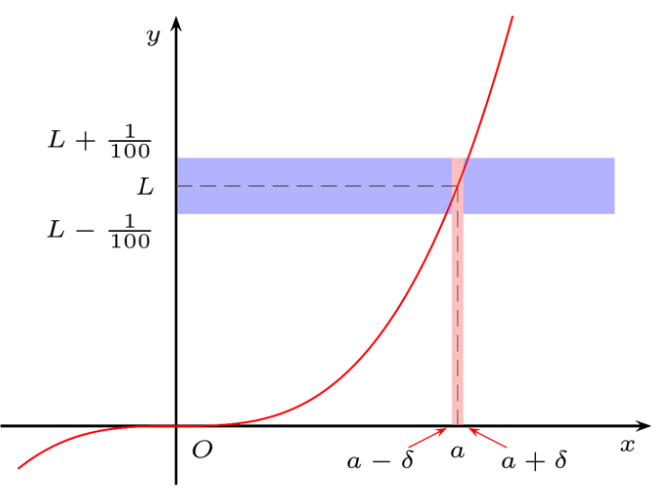
\includegraphics[width=0.8\linewidth]{ma1102r-limits.png}
\end{center}
informally,
\begin{itemize}
    \item $0 < \abs{x - a} < \delta \Then$ $x$ is close to but not equal to $a$.
    \item $0 < \abs{f(x) - L} < \epsilon \Then$ $f(x)$ is arbitrarily close to $L$.
\end{itemize}
% \begin{center}
%     if $f(x)$ is arbitrarily close to L by taking $x$ to be sufficiently close (but not equal to) $a$, then we write
%     \\* $\displaystyle{\lim_{x \to a} f(x) = L}$
%     \\* or $x \to a \Then f(x) \to L$
% \end{center}
% \begin{itemize}
%     \item the limit $\displaystyle{\lim_{x \to a} f(x)}$
%     \begin{itemize}
%         \item depends only on the values of $f(x)$ for $x$ near $a$    
%         \item is independent to the value of $f(x)$ at $a$.
%     \end{itemize}
% \end{itemize}

\subsection{limit laws}
\begin{tightcenter}
    \noindent\fbox{%
    \parbox{0.8\linewidth}{%
        you cannot apply any laws on limits 
        UNLESS you have shown that the limit exists!!
        }
    }%
\end{tightcenter}
\begin{itemize}
    \item Let $c \in \mathbb{R}$. $\displaystyle{\lim_{x \to a} c = c}$
    \item $\displaystyle{\lim_{x \to a} x = a}$
\end{itemize}
Suppose $\displaystyle{\lim_{x \to a} f(x) = L}$ and $\displaystyle{\lim_{x \to a} g(x) = M}$. Let $c$ be a constant. 
\begin{itemize}
    \item $\displaystyle{\lim_{x \to a} \left( cf(x) \right)} = cL = c \lim_{x \to a} f(x)$
    \item $\displaystyle{\lim_{x \to a} \left( f(x) + g(x) \right) = L + M = \lim_{x \to a} f(x) + \lim_{x \to a} g(x)}$
    \item $\displaystyle{\lim_{x \to a} \left( f(x) - g(x) \right) = \lim_{x \to a} f(x) - \lim_{x \to a} g(x)}$
    \item $\displaystyle{\lim_{x \to a} \left(f(x) g(x)\right) = \lim_{x \to a} f(x) \lim_{x \to a} g(x)}$
    \item $\displaystyle{\lim_{x \to a} \frac{f(x)}{g(x)} = \frac{\lim_{x \to a} f(x)}{\lim_{x \to a} g(x)}}$ provided that $\displaystyle{\lim_{x \to a} g(x) \neq 0}$
    \item $\displaystyle{\lim_{x \to a} \left( f(x) \right) ^n = \left(\lim_{x \to a} f(x)\right)^n}$
    \item $\displaystyle{\lim_{x \to a} \sqrt[n]{f(x)} = \sqrt[n]{\lim_{x \to a} f(x)}}$
\end{itemize}

\begin{center}
    \fbox{
        if $\displaystyle{\lim_{x \to a} \frac{f(x)}{g(x)}}$ exists and $\displaystyle{\lim_{x \to a} g(x) = 0}$, then $\displaystyle{\lim_{x \to a} f(x) = 0}$
    }
\end{center}

\subsubsection{inequalities on limits}
Suppose $\displaystyle{\lim_{x \to a} f(x) = L}$ and $\displaystyle{\lim_{x \to a} g(x) = M}$. 
\begin{center}
    \textbf{lemma}
    \\* if $f(x) \leq g(x)$ for all $x$ near $a$ (except possibly at $a$), 
    \\* then $L \leq M$.

    \textbf{lemma}
    \\* If $f(x) \geq 0$ for all $x$, then $L \geq 0$.
\end{center}

\subsubsection{direct substitution property}
Let $f$ be a polynomial or rational function. 
\begin{center}
    If $a$ is in the domain of $f$, then
    \\* $\displaystyle{\lim_{x \to a} f(x) = f(a)}$

    If $f(x) = g(x)$ for all $x$ near $a$ except possibly at $a$, then 
    \\* $\displaystyle{\lim_{x \to a} f(x) = \lim_{x \to a} g(x)}$
\end{center}

If $a$ is not in the domain (e.g. 0 denominator), don't apply directly - convert to an equivalent function and then sub in

\subsection{one-sided limits}
\begin{itemize}
    \item limit laws also hold for one-sided limits
\end{itemize}
\begin{center}
    If as $x$ is close to $a$ from the right, $f(x)$ is close to L, the right-hand limit of $f$ as $x$ approaches $a$ equals $L$.
    \\* $\displaystyle{\left( x \to a^+ \Then f(x) \to L \right) \Then \lim_{x \to a^+} f(x) = L}$
    \\ \ 
    \\ If as $x$ is close to $a$ from the left, $f(x)$ is close to L, the left-hand limit of $f$ as $x$ approaches $a$ equals $L$.
    \\* $\displaystyle{\left( x \to a^- \Then f(x) \to L \right) \Then \lim_{x \to a^-} f(x) = L}$
\end{center}
\begin{center}
    \fbox{
        $\displaystyle{\lim_{x \to a} f(x) = L \iff \lim_{x \to a^+} f(x) = \lim_{x \to a^-} f(x) = L}$
    }
    $f(x) \to L \Leftarrow x \to a \Iff \begin{cases}
        x \to a^+ \Then f(x) \to L \\
        x \to a^- \Then f(x) \to L
    \end{cases}$
\end{center}

\subsubsection{definition of one-sided limits}
\begin{center}
    \textbf{LH Limit}: $\displaystyle{\lim_{x \to a^-} f(x) = L}$ 
    \\* if for every $\epsilon > 0$ there exists $\delta > 0$ such that
    \\* $0 < a - x < \delta \Then \abs{f(x) - L} < \epsilon$
    \\ \ 
    \\ \textbf{RH Limit}: $\displaystyle{\lim_{x \to a^+} f(x) = L}$ 
    \\* if for every $\epsilon > 0$ there exists $\delta > 0$ such that
    \\* $0 < x - a < \delta \Then \abs{f(x) - L} < \epsilon$
\end{center}

\subsection{definition of infinite limits}
\begin{center}
    $\displaystyle{\lim_{x \to a} f(x) = \infty}$ 
    \\* if for every $M > 0$ there exists $\delta > 0$ such that
    \\* $0 < \abs{x - a} < \delta \Then f(x) > M$
    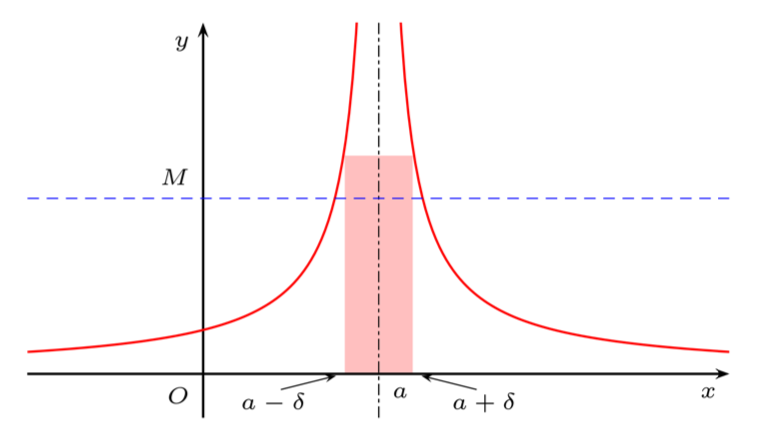
\includegraphics[width=0.7\linewidth]{ma1102r-infinite-limit.png}
    \\* \textbf{negative infinite limit:}
    \\* $0 < \abs{x - a} < \delta \Then f(x) < M$
\end{center}
\begin{itemize}
    \item $\infty$ is NOT a number $\Then$ an infinite limit does NOT exist
\end{itemize}

\subsubsection{limits to infinity}
Suppose $f$ is defined on $[M, \infty)$ for some $M \in \mathbb{R}$:
\begin{center}
    $\displaystyle{\lim_{x \to \infty}f(x) = L}$: 
    \\* For every $\epsilon > 0$, there exists $N$ such that
    \\* $x > N \Then \abs{f(x) - L} < \epsilon$
    \\ \ 
    \\ $\displaystyle{\lim_{x \to \infty}f(x) = \infty}$: 
    \\* For every $M > 0$, there exists $N$ such that
    \\* $x > N \Then f(x) > M$
\end{center}
% \begin{center}
%     Suppose $f$ is defined on both sides of $a$ (except possibly at $a$).
%     \\* If $f(x)$ is arbitrarily large by taking $x$ sufficiently close to $a$, 
%     \\* $\displaystyle{\lim_{x \to a} f(x) = \infty}$
%     \\* If $f(x)$ is arbitrarily negatively large $\cdots$, 
%     \\* $\displaystyle{\lim_{x \to a} f(x) = -\infty}$

%     Suppose $f$ is defined on $[M, \infty)$ for some real number $M$.
%     \\* If $f(x)$ is arbitrarily close to $L$ by taking $x$ sufficiently large,
%     \\* $\displaystyle{\lim_{x \to \infty} f(x) = L}$
% \end{center}

\subsection{squeeze theorem}
Suppose $f(x)$ is bounded by $g(x)$ and $h(x)$ where 
    \begin{itemize}
        \item $g(x) \leq f(x) \leq h(x)$ for all $x$ near $a$ (except at $a$), and
        \item $\displaystyle{\lim_{x \to a} g(x) = \lim_{x \to a} h(x) = L}$.
    \end{itemize}
\begin{center}
    Then $\displaystyle{\lim_{x \to a} f(x) = L}$.
    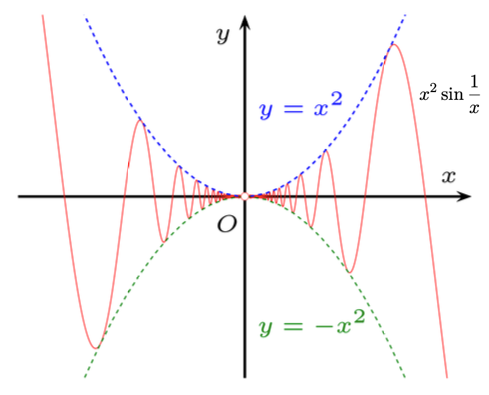
\includegraphics[width=0.8\linewidth]{ma1102r-squeeze-theorem.png}
\end{center}


\section{02. CONTINUOUS FUNCTIONS}
\subsection{definition of continuity}
\begin{center}
    a function $f$ is \textbf{continuous at $a$} $\iff$ 
    \\* $f$ is continuous from the left and from the right at $a$.
    \\* $\displaystyle{\lim_{x \to a} f(x) = f(a)}$
    \begin{itemize}
        \item $f$ is continuous from the right at $a$ if $\displaystyle{\lim_{x \to a^+} f(x) = a}$
        \item $f$ is continuous from the left at $a$ if $\displaystyle{\lim_{x \to a^-} f(x) = a}$
    \end{itemize}
\end{center}

a function $f$ is \textbf{continuous at an interval} if it is continuous at every number in the interval.
\begin{center}
    $f$ is continuous on \textbf{open interval} $(a, b)$
    \\* $\Iff f$ is continuous at every $x \in (a, b)$
    \\ $f$ is continuous on \textbf{closed interval} $[a, b]$
    $\Iff \begin{cases}
        f $ is continuous at every $x \in (a, b) \\
        f $ is continuous from the right at $ a \\
        f $ is continuous from the left at $ b
    \end{cases}$
\end{center}

\subsubsection{precise definition of continuity}
\begin{center}
    a function $f$ is \textbf{continuous} at a number $a$ if 
    \\* for all $\epsilon > 0$, there exists $\delta > 0$ such that 
    $\abs{x - a} < \delta \Then \abs{f(x) - f(a)} < \epsilon$
\end{center}
\begin{itemize}
    \item aka $\displaystyle{\lim_{x \to a}} f(x) = f(a)$
\end{itemize}

\subsubsection{continuity test}
$f$ is continuous at $a \Iff$ 
\begin{enumerate}
    \item $f$ is defined at $a$ ($a$ is in the domain of $f$)
    \item $\displaystyle{\lim_{x \to a} f(x)}$ exists
    \item $\displaystyle{\lim_{x \to a} f(x)} = f(a)$ 
\end{enumerate}

\subsubsection{examples of discontinuity}
\begin{center}
    \begin{multicols*}{3}
        removable
        \\* 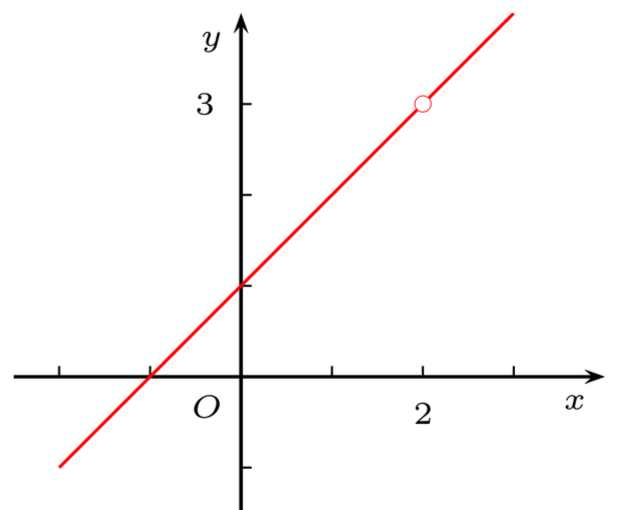
\includegraphics[width=0.95\linewidth]{ma1102r-removable-discontinuity.png}
        infinite
        \\* 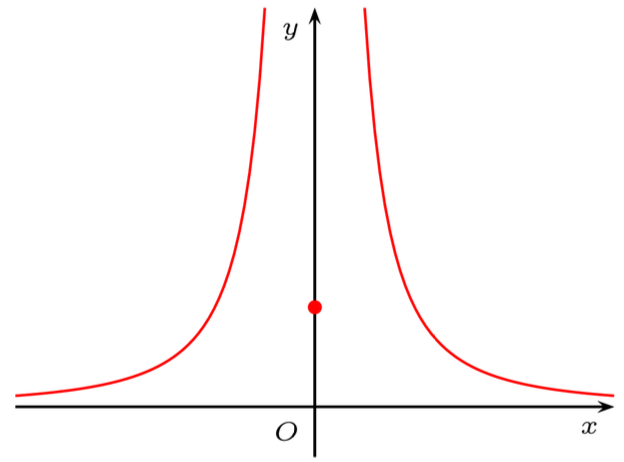
\includegraphics[width=0.95\linewidth]{ma1102r-infinite-discontinuity.png}
        jump
        \\* 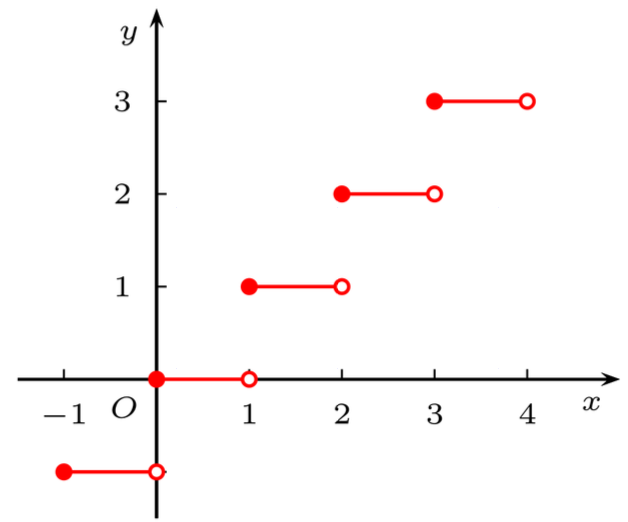
\includegraphics[width=0.95\linewidth]{ma1102r-jump-discontinuity.png}
    \end{multicols*}
\end{center}

\subsection{properties of continuous functions}
let $f$ and $g$ be functions continuous at $a$. let $c$ be a constant.
\begin{enumerate}
    \item $cf$ is continuous at $a$
    \item $f+g$ is continuous at $a$
    \item $f-g$ is continuous at $a$
    \item $fg$ is continuous at $a$
    \item $f/g$ is continuous at $a$, provided $g(a) \neq 0$
\end{enumerate}

\textbf{other properties}
\begin{itemize}
    \item a polynomial is continuous everywhere
    \item a rational function is continuous on its domain
    \begin{itemize}
        \item if $P(x)$ and $Q(x)$ are polynomials, $\frac{P(x)}{Q(x)}$ is continuous whenever $Q(x) \neq 0$.
    \end{itemize}
    \item $f(x) = c$ is continuous on $\mathbb{R}$ for all $c \in \mathbb{R}$.
    \item $f(x) = x$ is continuous on $\mathbb{R}$.
\end{itemize}

\subsubsection{trigonometric functions}
\begin{itemize}
    \item $f(x) = \sin x$  and $g(x) = \cos x$ are continuous everywhere
    \item $\tan x, \sec x$ are continuous whenever $\cos x \neq 0$
    \begin{itemize}
        \item domain: $\mathbb{R} \backslash \{\pm \frac{pi}{2}, \pm \frac{3\pi}{2}, \pm \frac{5\pi}{2}, \dots\}$
    \end{itemize}
    \item $\cot x, \csc x$ are continuous whenever $\sin x \neq 0$
    \begin{itemize}
        \item domain: $\mathbb{R} \backslash \{0, \pm \pi, \pm 2\pi, \cdots\}$
    \end{itemize}
\end{itemize}

\subsection{composite of continuous functions}
\begin{center}
    if $f$ is continuous at $b$ and $\displaystyle{\lim_{x \to a} g(x) = b}$, then 
    \\* $\displaystyle{\lim_{x \to a} f(g(x)) = f(\lim_{x \to a} g(x)) = f(b)}$
\end{center}
\begin{center}
    if $g$ is continuous at $a$ and $f$ is continuous at $g(a)$,
    \\* then $f \circ g$ is continuous at $a$.
    \\* $\displaystyle{\lim_{x \to a} (f \circ g)(x) = (f \circ g)(a)}$
\end{center}

\subsection{substitution theorem}
Suppose $y = f(x)$ such that $\displaystyle{\lim_{x \to a}f(x) = b}$. If
\begin{enumerate}
    \item $g$ is continuous at $b$, OR 
    \item $\forall x$ near $a$, except at $a$, $f(x) \neq b$ and $\displaystyle{\lim_{y \to b} g(y)}$ exists
    \begin{itemize}
        \item aka, $\displaystyle{\lim_{y \to b}g(y)}$ exists and $f$ is one-to-one.
    \end{itemize}
\end{enumerate}
Then $\displaystyle{\lim_{x \to a} g(f(x)) = \lim_{y \to b} g(y)}$

\subsection{intermediate value theorem}\
\begin{center}
    Let $f$ be a function continuous on $[a, b]$ with $f(a) \neq f(b)$. 
    \\* Let $N$ be a number between $f(a)$ and $f(b)$.
    \\* Then there exists $c \in (a, b)$ such that $f(c) = N$.
    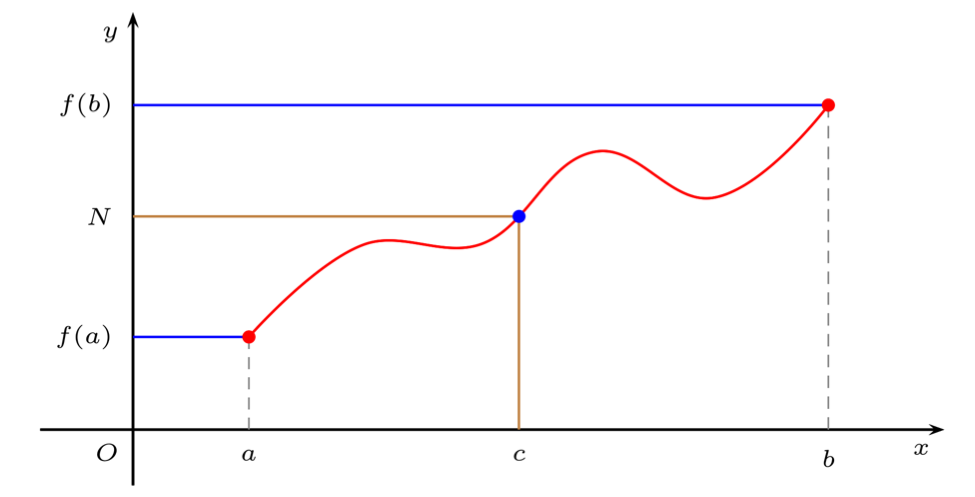
\includegraphics[width=0.9\linewidth]{ma1102r-intermediate-value-theorem.png}
\end{center}

\section{03. DERIVATIVES}

\subsection{tangent line}
\begin{center}
    the \textbf{tangent line} to $y=f(x)$ at $(a, f(a))$ is 
    \\* the line passing through $(a, f(a))$ with slope $f'(a)$:
    \fbox{
        $y = f'(a)(x-a) + f(a)$
    }
\end{center}

\subsection{definition of derivatives}
\begin{itemize}
    \item $f$ is differentiable at $a$ if $f'(a)$ exists
    \item $f'(a)$ is the slope of $y=f(x)$ at $x=a$
    \begin{itemize}
        \item $f'(a) = \frac{dy}{dx}\vert_{x = a}$
        \item $\frac{dy}{dx} := {\displaystyle\lim_{x \to 0}} \frac{\Delta y}{\Delta x}$  (derivative of $y$ with respect to $x$)
    \end{itemize}
    \item $f'(x) = y' = \frac{dy}{dx} = \frac{df}{dx} = \frac{d}{dx}f(x) = D_xf(x) = \cdots$
\end{itemize}
\begin{tightcenter}
    \noindent\fbox{%
        \parbox{0.9\linewidth}{%
            \begin{tightcenter}
            the \textbf{derivative} of a function $f$
            \\* ${\displaystyle{f'(x) := \lim_{h \to 0}}} \frac{f(x+h) - f(x)}{h}$
            \\ the \textbf{derivative} of a function $f$ at a number $a$ is 
            \\* ${\displaystyle{f'(a) := \lim_{x \to a}}} \frac{f(x) - f(a)}{x-a}$
            \end{tightcenter}
            }
        }%
\end{tightcenter}

\subsection{differentiable functions}
\begin{itemize}
    \item $f$ is differentiable at $a$ if 
    \begin{itemize}
        \item ${\displaystyle{f'(a) := \lim_{x \to 0}}}\frac{f(a + h) - f(a)}{h}$ exists.
    \end{itemize}
    \item $f$ is differentiable on $(a, b)$ if 
    \begin{itemize}
        \item $f$ is differentiable at every $c \in (a, b)$
    \end{itemize}
\end{itemize}

\subsubsection{differentiability \& continuity}
\begin{itemize}
    \item differentiability $\Then$ continuity
    \begin{itemize}
        \item if $f$ is differentiable at $a$, then $f$ is continuous at $a$.
    \end{itemize}
    \item continuity $\nRightarrow$ differentiability
\end{itemize}

\subsection{differentiation}
\begin{itemize}
    \item every polynomial and rational function is differentiable on its domain
    \begin{itemize}
        \item the domain of $f'$ may be smaller than the domain of $f$.
    \end{itemize}
    \item trigonometric functions are differentiable on the domain
\end{itemize}

\subsubsection{differentiation of trigonometric functions}
\begin{center}
    \begin{multicols}{2}
        ${\displaystyle{\lim_{\theta \to 0}} \frac{\sin\theta}{\theta} = 1}$
        \\ ${\displaystyle{\lim_{\theta \to 0}} \frac{1 - \cos\theta}{\theta} = 0}$
    \end{multicols}
\end{center}

\subsubsection{chain rule}
\begin{center}
    If $g$ is differentiable at $a$ and $f$ is differentiable at $b = g(a)$, then $F = f \circ g$ is differentiable at $a$ and
    \\* $F'(a) = (f \circ g)'(a) = f'(b)g'(a) = f'(g(a))g'(a)$
\end{center}
\begin{center}
    If $z=f(y)$ and $y = g(x)$, then 
    \\* $\frac{dz}{dx} = \frac{dz}{dy} \frac{dy}{dx}$
    \\* $\frac{dz}{dx}\vert_{x=a} = \frac{dz}{dy}\vert_{y=b} \frac{dy}{dx}\vert_{x=a}$
\end{center}

\subsubsection{generalised chain rule}
$h$ is differentiable at $a$; $g$ is differentiable at $B = h(a)$; $f$ is differentiable at $c = g(b)$.
\begin{align*}
    (f \circ (g \circ h))'&= f' \circ (g \circ h) \cdot (g \circ h)'
    \\ &= f'(c)g'(b)h'(a)
\end{align*}
\begin{center}
    Leibniz notation:
    \\* If $y = h(x), z=g(y), w=f(z)$,
    \\* $\frac{dw}{dx}  = \frac{dw}{dz} \frac{dz}{dy} \frac{dy}{dx}$
\end{center}

\subsection{implicit differentiation}
\begin{itemize}
    \item assumes that $\frac{dy}{dx}$ exists
\end{itemize}

\subsection{second derivative}
\begin{center}
    $f''(x) = \frac{d}{dx}(\frac{dy}{dx}) = \frac{d^2y}{dx^2}$
    \\* $f' = D(f) \Rightarrow f'' := D^2(f)$
\end{center}

\subsection{higher derivatives}
\begin{center}
    $f^{(0)} := f$
    \\* For any positive integer $n$, $f^{(n)} := (f^{(n-1)})'$
    \\* if $y=f(x)$, then $f^{(n)}(x) = y^{(n)} = \frac{d^ny}{dx^n} = D^nf(x)$
\end{center}
\begin{itemize}
    \item for $f(x) = \frac{1}{x}$, $f^{(n)}(x) = \frac{(-1)^nn!}{x^{n+1}}$
    \item for $f(x) = x^m$, $f^{(n)}(x) = \begin{cases}
        \frac{m!x^{m-n}}{(m-n)!} &\text{ if } m \geq n,
        \\ 0 &\text{ if } m < n.
    \end{cases}$
\end{itemize}

\section{04. APPLICATIONS OF DIFFERENTIATION}

\subsection{extreme values of functions}
Let $f$ be a function with domain $D$.

\subsubsection{global (absolute) max/min}
\begin{itemize}
    \item aka absolute max/min
    \item extreme values = absolute maximum and absolute minimum
\end{itemize}
\begin{center}
    $f$ has a global \textbf{maximum} at $c \in D$
    \\* $\Iff f(c) \geq f(x)$ for all $x \in D$
    \\ $f$ has a global \textbf{minimum} at $c \in D$
    \\* $\Iff f(c) \leq f(x)$ for all $x \in D$
\end{center}

\subsubsection{local max/min}
\begin{itemize}
    \item aka relative max/min aka "turning points"
    \item "all $x$ near $c$" = for all $x$ in an open interval containing $c$
\end{itemize}
\begin{center}
    $f$ has a local \textbf{maximum} at $c \in D$ 
    \\* $\Iff f(c) \geq f(x)$ for all $x$ near $c$
    \\ $f$ has a local \textbf{minimum} at $c \in D$ 
    \\* $\Iff f(c) \leq f(x)$ for all $x$ near $c$
\end{center}
\begin{itemize}
    \item local max/min $\nRightarrow$ global max/min
    \item global max/min $\nRightarrow$ local max/min
\end{itemize}

\subsection{extreme value theorem}
\begin{center}
    \textbf{existence}
    \\* if $f$ is \textit{continuous} on a \textit{finite closed} interval $[a, b]$,
    \\* then $f$ attains extreme values on $[a, b]$.

    \textbf{value}
    \\* the extreme value occurs at either 
    \\* \textit{critical numbers} or the \textit{endpoints} ($x=a, x=b$).
\end{center}

\subsection{critical numbers}
\begin{center}
    $c \in D$ is a \textit{critical number} of $f$ if 
    \\* $f'(c) = 0$, or $f'(c)$ does not exist.
\end{center}
\begin{center}
    \textbf{fermat's theorem}
    \\* If $f$ has a local maximum or minimum at $c$, 
    \\* then $c$ is a critical number.
    \\* If $f'(c)$ exists, then $f'(c)=0$.
\end{center}

\subsection{Rolle's Theorem}
\begin{center}
    Let $f$ be a function such that $f$ is \textit{continuous} on $[a, b]$, $f$ is \textit{differentiable} on $(a, b)$, and $f(a) = f(b)$.
    \\* Then there is a number $c \in (a, b)$ such that $f'(c) = 0$.
\end{center}

\subsection{mean value theorem}
\begin{center}
    Let $f$ be a function such that 
    \\* $f$ is \textit{continuous} on $[a, b]$ and $f$ is \textit{differentiable} on $(a, b)$.
    \\* Then there exists $c \in (a, b)$ such that 
    \\* $f'(c) = \frac{f(b) - f(a)}{b-a}$
\end{center}
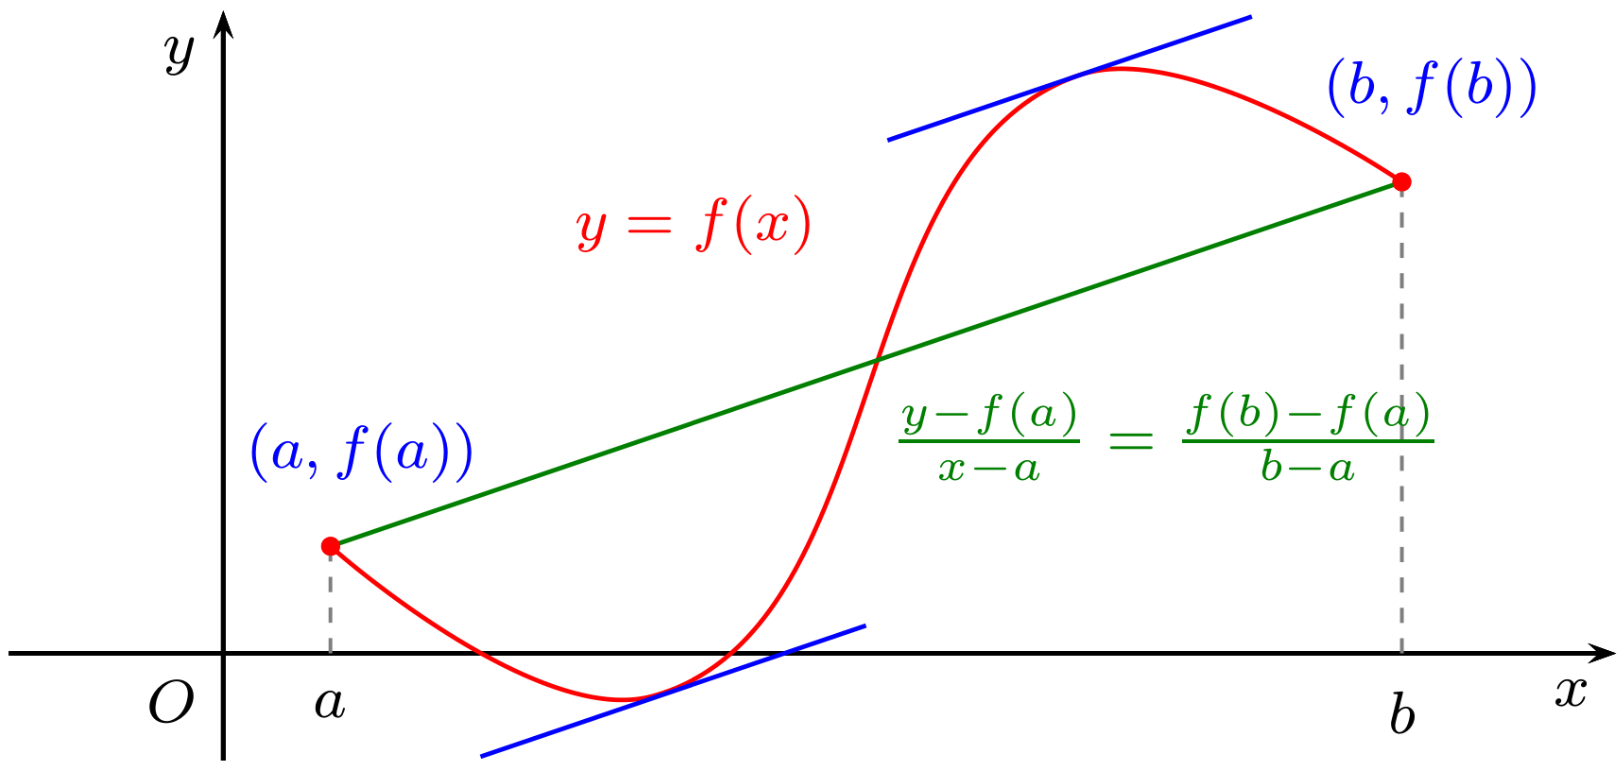
\includegraphics[width=0.9\linewidth]{ma1102r-mean-value-theorem.png}
\begin{itemize}
    \item generalisation of Rolle's theorem when $f(a) = f(b)$.
\end{itemize}

\subsubsection{ordinary differential equations}
\begin{center}
    Let $f$ and $g$ be continuous on $[a, b]$.
    \\* If $f'(x) = g'(x)$ for all $x \in (a, b)$, 
    \\* then $f(x) = g(x) + C$ on $[a, b]$ for a constant $C$.
\end{center}

\subsection{increasing/decreasing test}
Let $f$ be continuous on $[a, b]$ and differentiable on $(a, b)$.
\begin{itemize}
    \item $f'(x) > 0$ for any $x \in (a, b) \Then f$ is increasing.
    \begin{itemize}
        \item $f$ is increasing $\Then f(x) \geq 0$
    \end{itemize}
    \item $f'(x) < 0$ for any $x \in (a, b) \Then f$ is decreasing.
    \begin{itemize}
        \item $f$ is decreasing $\Then f(x) \leq 0$
    \end{itemize}
    \item $f'(x) = 0 \Then f$ could be increasing OR decreasing.
\end{itemize}

\subsection{first derivative test}
Let $f$ be continuous and $c$ be a critical number of $f$. Suppose $f$ is differentiable near $c$ (except possibly at $c$).
At $c$, if $f'$ changes from:
\begin{itemize}
    \item (+) to (-) $\then f$ has a local \textbf{maximum} at $c$
    \item (-) to (+) $\then f$ has a local \textbf{minimum} at $c$
    \item no change in sign $\then f$ has neither local max/min at $c$.
\end{itemize}

\subsection{concavity}
\begin{center}
    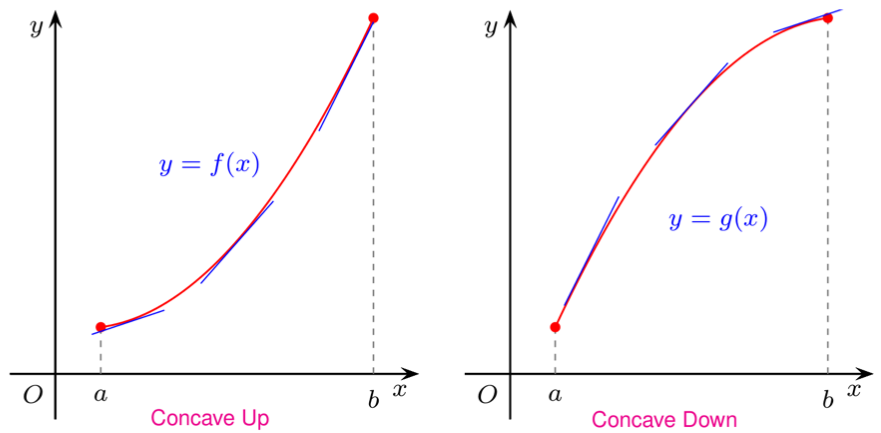
\includegraphics[width=0.8\linewidth]{ma1102r-concavity.png}
    \\ $f$ is \textbf{concave up} on an open interval $I$ 
    \\* if $f(x) > f'(y)(x-y) + f(y)$ for any $x \neq y \in I$
    \\* for $a < b \in I$, $f'(a) < f'(b)$
    \\* concave up $\Iff f'$ is increasing

    $f$ is \textbf{concave down} on an open interval $I$
    \\* if $f(x) < f'(y)(x-y) + f(y)$ for any $x \neq y \in I$
    \\* for $a < b \in I$, $f'(a) > f'(b)$
    \\* concave down $\Iff f'$ is decreasing

    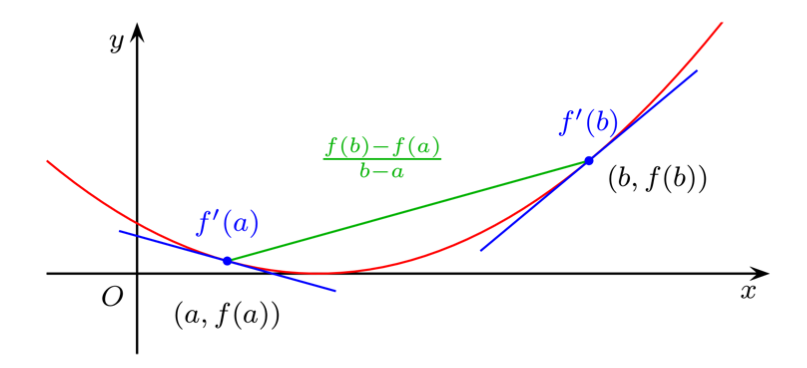
\includegraphics[width=0.9\linewidth]{ma1102r-concavity-shortcut.png}
\end{center}

\subsubsection{concavity test}
\begin{itemize}
    \item $f'' > 0$ on $I \Then f$ is concave up on $I$
    \item $f'' < 0$ on $I \Then f$ is concave down on $I$
\end{itemize}

\subsection{second derivative test}
If $f'(c) = 0$ and $f''(c)$ exists,
\begin{itemize}
    \item $f''(c) < 0 \Then f$ has a \textbf{local maximum} at $c$.
    \item $f''(c) > 0 \Then f$ has a \textbf{local minimum} at $c$.
    \item $f''(c) = 0 \Then$ inconclusive
\end{itemize}

\subsection{inflection point}
\begin{itemize}
    \item A point $P$ on the curve $y = f(x)$ is an inflection point if
    \begin{itemize}
        \item $f$ is continuous at $P$, and
        \item the concavity of the curve changes at $P$.
    \end{itemize}
    \item if $c$ is an inflection point and $f$ is twice differentiable at $c$, then $f''(c) = 0$.
\end{itemize}

\subsection{Taylor's Theorem}
\begin{center}
    $f(x) = f(a) + f'(a)(x-a) + \frac{f''(a)}{2}(x-a)^2 + \dots + \frac{f^{(n)}(a)}{n!}(x-a)^n + R_n,$
    \\* where $R_n = \frac{f^{(n+1)}(a)}{(n+1)!}(x-a)^{(n+1)}$ for $c$ between $x$ and $a$
\end{center}
\subsubsection{Taylor Series}
\begin{center}
    As $R-n \to 0$ as $n \to \infty$, then
    \\* $\displaystyle{f(x) = \sum^\infty_{n=0} \frac{f^{(n)}(a)}{n!}(x-a)^n}$
\end{center}

\subsection{L'Hopital's Rule $(\frac{0}{0})$}
Let $f$ and $g$ be functions such that 
\begin{itemize}
    \item $\displaystyle{\lim_{x \to a}f(x) = \lim_{x \to a}g(x) = 0}$ 
    \item $f$ and $g$ are differentiable near $a$ (except at $a$).
\end{itemize}
\begin{tightcenter}
    Then $\displaystyle{\lim_{x \to a}\frac{f(x)}{g(x)} = \lim_{x \to a}\frac{f'(x)}{g'(x)}}$,
    \\* provided that the RHS limit exists or is $\pm \infty$
\end{tightcenter}

\subsection{L'Hopital's Rule $(\frac{\infty}{\infty})$}
Suppose that 
\begin{itemize}
    \item $\displaystyle{\lim_{x \to a}\abs{f(x)} = \lim_{x \to a}\abs{g(x)} = \infty}$,
    \item $f$ and $g$ are differentiable near $a$ (except at $a$), 
    \item $g'(x) \neq 0$ near $a$ (except at $a$)
\end{itemize}
\begin{tightcenter}
    Then $\displaystyle{\lim_{x \to a}\frac{f(x)}{g(x)} = \lim_{x \to a}\frac{f'(x)}{g'(x)}}$
    \\ provided that the RHS limit exists or is $\pm \infty$
\end{tightcenter}

\subsection{Cauchy's Mean Value Theorem}
\begin{center}
    Let $f, g$ be continuous on $[a, b]$, differentiable on $(a, b)$, 
    \\* and $g'(x) \neq 0$ for any $x \in (a, b)$.
    \\* Then there exists $c \in (a, b)$ such that 
    \\* $\frac{f'(c)}{g'(c)} = \frac{f(b) - f(a)}{g(b) - g(a)}$
    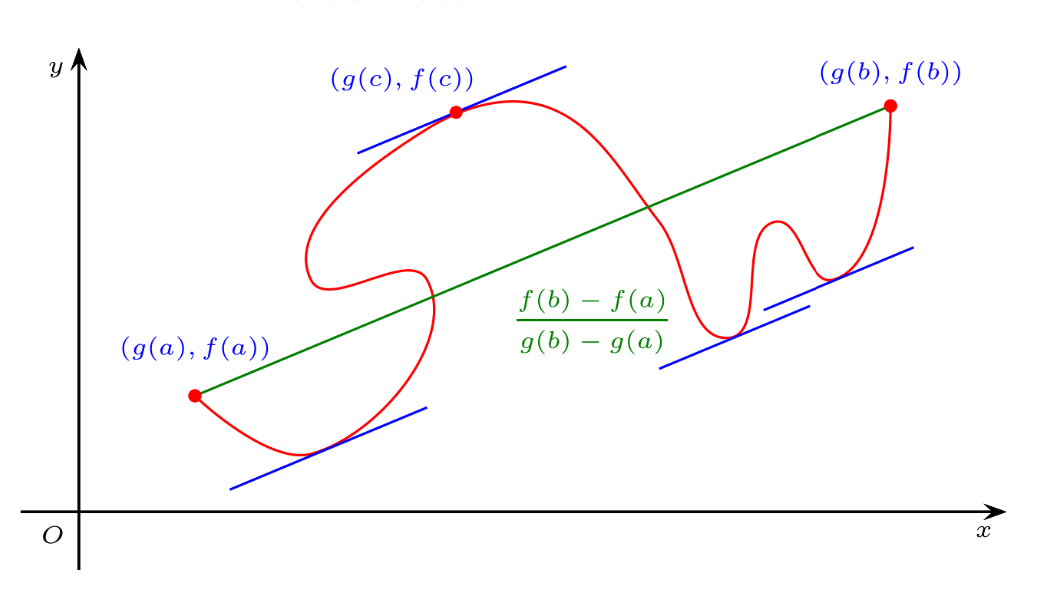
\includegraphics[width=0.9\linewidth]{ma1102r-cauchy-mvt.png}
\end{center}

\section{05. INTEGRALS}
\subsection{definite integral}
Let $f$ be a continuous function on $[a, b]$ divided into $n$ intervals.
\begin{center}
    \textbf{Riemann sum}
    \\* $\left[ f(x_1^*) + f(x_2^*) + \cdots + f(x^*_n) \right] \Delta x = {\displaystyle\sum^n_{i=1}f(x_i^*)\Delta x}$
    \begin{itemize}
        \item the lengths of subintervals are not necessarily equal
        \begin{itemize}
            \item $\max\{\abs{x_i - x_{i-1} : i = 1, \cdots, n}\} \to 0$
        \end{itemize}
    \end{itemize}
\end{center}

\begin{center}
    \textbf{definite integral} of $f$ from $a$ to $b$:
    \noindent\fbox{%
    \parbox{0.9\linewidth}{%
    \begin{tightcenter}
        ${\displaystyle{\int^b_a f(x) dx = \lim_{n \to \infty} \sum^n_{i = 1} f(x_i^*) \Delta x}}$
    \end{tightcenter}
    }
    }%
    \\* where $\Delta x = \frac{b - a}{n}$
\end{center}
\begin{itemize}
    \item $f$ is \textbf{integrable} from $a$ to $b$ if ${\displaystyle{\lim_{n \to \infty} \sum^n_{i = 1} f(x_i^*) \Delta x}}$ exists.
    \item continuous functions are integrable.
    \item $\int^b_a f(x) dx = - \int^a_b f(x) dx$
    \item $\int^a_a f(x) dx = 0$
\end{itemize}

\subsubsection{properties}
let $f$ and $g$ be continuous functions.
\begin{itemize}
    \item $\int^b_a c \dx = (b-a) c$
    \item $\int^b_a (f(x) \pm g(x)) \dx = \int^b_a f(x) \dx \pm \int^b_a g(x) \dx$
    \item $\int^c_a f(x) \dx = \int^c_b f(x) \dx \pm \int^b_a f(x) \dx$
    \item suppose $f(x) \geq 0$ on $[a, b]$. Then $\int^b_a f(x) \dx \geq 0$.
    \item suppose $f(x) \geq g(x)$ on $[a, b]$. 
    \item \begin{itemize}
        \item Then $\int^b_a f(x) \dx \geq \int^b_a g(x) \dx$.
    \end{itemize}
    \item suppose $m \leq f(x) \leq M$ on $[a, b]$. 
    \begin{itemize}
        \item Then $m(b - a) \leq \int^b_af(x) \dx \leq M(b-a)$.
    \end{itemize}
\end{itemize}

\subsection{fundamental theorem of calculus}
for $g(x) = \int^x_a f(t) \, dt \quad (a \leq x \leq b)$, 
\begin{itemize}
    \item $g$ is continuous on $[a, b]$
    \item $g$ is differentiable on $(a, b)$
    \item $g'(x) = f(x)$ on $(a, b) \quad$ or $\quad \frac{d}{dx} \int^x_a f(t) \mathop{dt} = f(x)$
\end{itemize}
\begin{tightcenter}
    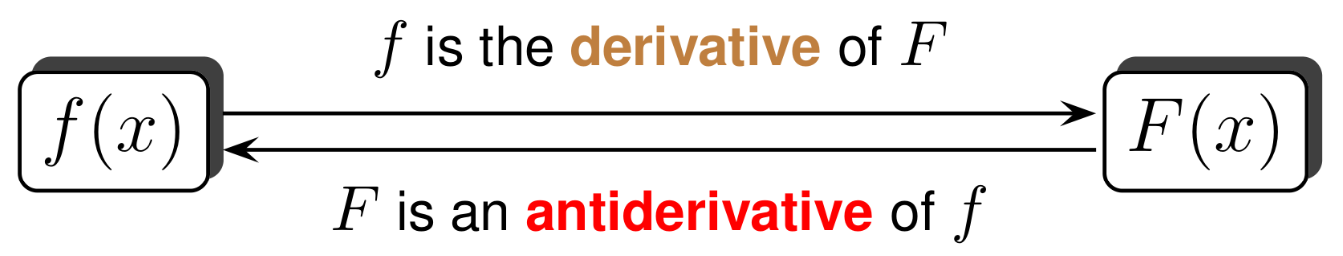
\includegraphics[width=0.7\linewidth]{ma1102r-derivatives.png}
\end{tightcenter}
if $F$ is continuous on $[a, b]$, and $F' = f$ on $(a, b)$,
\begin{tightcenter}
    ${\displaystyle{\int^b_a f(x) \dx = F(b) - F(a) = F(x) \Bigr|^{x = b}_{x = a}}}$
    \\* ${\displaystyle{\int^x_a \frac{d}{dx} F(t) \mathop{dt} = F(x) - F(a)}}$
    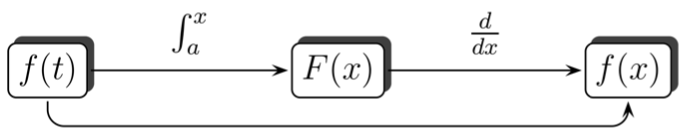
\includegraphics[width=0.7\linewidth]{ma1102r-ftc-1.png}
    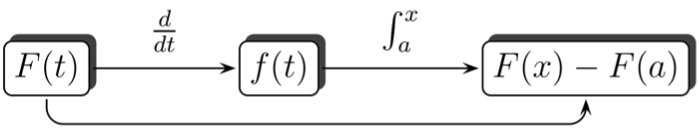
\includegraphics[width=0.7\linewidth]{ma1102r-ftc-2.png}
\end{tightcenter}

\subsection{indefinite integral}
\begin{itemize}
    \item \textbf{indefinite integral} of $f$, ${\displaystyle{\int f(x) \dx = F(x) + c}}$
    \item \textbf{antiderivative} (of a continuous function $f$): a continuous function $F$ such that $F' = f$.
    \begin{itemize}
        \item antiderivatives of $f$ are functions of form $F + c$
        \item indefinite integral is a family of antiderivatives
    \end{itemize}
    \item properties of indefinite integral
    \begin{itemize}
        \item ${\displaystyle{\int (af(x) \pm bg(x)) \dx = a \int f(x) \dx \pm \, b \int g(x) \dx}}$
    \end{itemize}
\end{itemize}

\subsection{integration by parts}
\begin{center}
    ${\displaystyle{u \mathop{dv} = uv - \int v \mathop{du}}}$
\end{center}

\subsection{substitution rule (I)}
let $u = g(x)$ be a differentiable function. 
\subsubsection{indefinite integral}
\begin{center}
    if $f$ and $g'$ are continuous, 
    \\* ${\displaystyle{\int f(g(x))g'(x) \dx = \int f(u) \mathop{du}}}$
\end{center}
\subsubsection{definite integral}
\begin{center}
    if $g'$ are continuous on $[a, b]$,
    \\* and $f$ is continuous on the range of $u = g(x)$,
    \\* ${\displaystyle{\int^b_a f(g(x))g'(x) \dx = \int^{g(b)}_{g(a)} f(u) \mathop{du}}}$
\end{center}

\subsection{substitution rule (II)}
let $f$ and $g'$ be continuous functions, and 
\\* $x = g(t)$ is a one-to-one differentiable function.
\begin{center}
    ${\displaystyle{\int f(x) \dx = \int f(g(t))g'(t) \mathop{dt}}}$
\end{center}


\subsection{improper integral}
\subsubsection{for discontinuous integrands}
\begin{center}
    if $f$ is continuous on $[a, b)$ and discontinuous at $b$,
    \\* ${\displaystyle{\int^b_a f(x) \dx = \lim_{t \to b^-} \int^t_a f(x) \dx}}$
\end{center}

\begin{center}
    if $f$ is continuous on $(a, b]$ and discontinuous at $a$,
    \\* ${\displaystyle{\int^b_a f(x) \dx = \lim_{t \to a^+} \int^b_t f(x) \dx}}$
\end{center}
\begin{itemize}
    \item $\int^b_a f(x) \dx$ is the limit of integrals.
    \begin{itemize}
        \item \textbf{converges} if the limit exists
        \item \textbf{diverges} if the limit does not exist
    \end{itemize}
\end{itemize}

\subsubsection{discontinuity in the interior of the interval}
\begin{center}
    suppose $f$ has discontinuity at $c \in (a, b)$. then
    \\* ${\displaystyle{\int^b_a f(x) \dx = \lim_{t \to c^-} \int^t_a f(x) \dx + \lim_{t \to c^+} \int^b_t f(x) \dx}}$ 
\end{center}

\subsubsection{over infinite intervals}
\begin{center}
    ${\displaystyle{\int^\infty_{-\infty} f(x) \dx = \int^a_{-\infty} f(x) \dx + \int^\infty_a f(x) \dx}}$
\end{center}

\begin{center}
    if $\int^t_a f(x) \dx$ exists for every $t \geq a$, then
    \\* the \textbf{improper integral} of $f$ from $a$ to $\infty$ is
    \\* ${\displaystyle{\int^\infty_a f(x) \dx = \lim_{t \to \infty} \int^t_a f(x) \dx}}$
\end{center}

\begin{center}
    if $\int^b_t f(x) \dx$ exists for every $t \leq b$, then
    \\* the \textbf{improper integral} of $f$ from $-\infty$ to $b$ is
    \\* ${\displaystyle{\int^\infty_a f(x) \dx = \lim_{t \to \infty} \int^t_a f(x) \dx}}$
\end{center}

\begin{itemize}
    \item NOTE: $\int^\infty_{-\infty} f(x) \dx \neq \lim_{a \to \infty} \int^a_{-a} f(x) \dx$
\end{itemize}


\begin{center}
    \ 
\end{center}

\section{06. INVERSE FUNCTIONS \& INTEGRATION}

\subsection{one to one functions}
\begin{center}
    let $f$ be a function with domain $D$. 
    \\* $f$ is \textbf{one-to-one} if, for any $a, b \in D$, 
    \\* $a \neq b \then f(a) \neq f(b)$
    \\* OR $f(a) = f(b) \then a = b$
\end{center}

\subsection{inverse function}
let $f$ be a one-to-one function with domain $A$ and range $B$.
\begin{itemize}
    \item its \textbf{inverse function} $f^{-1}$ is the function with
    \begin{itemize}
        \item domain $B$ and range $A$, and
        \item $f^{-1}(y) = x \iff y = f(x)$ for any $x \in A$, $y \in B$
    \end{itemize}
    \item $f^{-1} \circ f = id_A$ and $f \circ f^{-1} = id_B$
    \item $(f^{-1})^{-1} = f$
    \item NOTE: $(f(x))^{-1}$ is the reciprocal of the value of $f(x)$
\end{itemize}
\subsubsection{properties}
let $f$ be a \textit{one-to-one continuous} function on an open interval $I$.
\begin{itemize}
    \item the inverse function $f^{-1}$ is also continuous.
    \item if $f$ is differentiable at $a \in I$, and $f'(a) \neq 0$, then
    \begin{itemize}
        \item $f^{-1}$ is differentiable at $b = f(a)$
        \item $(f^{-1})'(b) = \frac{1}{f'(a)}$
    \end{itemize}
\end{itemize}
\begin{tightcenter}
    \noindent\fbox{%
    \parbox{0.5\linewidth}{%
    \begin{tightcenter}
        $(f^{-1})'(f(a)) = \frac{1}{f'(a)}$
    \end{tightcenter}
    }
    }%
    \\ 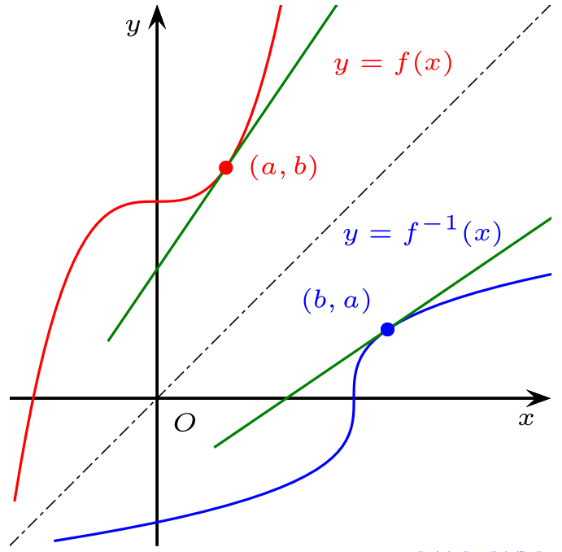
\includegraphics[width=0.5\linewidth]{ma1102r-inverse-functions.png}
\end{tightcenter}

\subsection{techniques of integration}
\subsubsection{common trigonometric substitutions}
\begin{itemize}
    \item $\sqrt{a^2 - x^2}, \quad x = a\sin t, \quad t \in [-\frac{\pi}{2}, \frac{\pi}{2}]$
    \item $\sqrt{x^2 - a^2}, \quad x = a\sec t, \quad t \in [0, -\frac{\pi}{2}) \cup (\pi, \frac{3\pi}{2}]$
    \item $a^2 + x^2, \quad x = a\tan t, \quad t \in (-\frac{\pi}{2}, \frac{\pi}{2})$
\end{itemize}

\subsubsection{integration of rational functions}
for $f = \frac{A(x)}{B(x)}$,
\begin{itemize}
    \item manipulate such that $\deg A(x) < \deg B(x)$, \\* then decompose into partial fractions
    \item common rational functions:
    \begin{itemize}
        \item ${\displaystyle{\int \frac{1}{(x+a)^k} \dx = \begin{cases}
            \ln \abs{x + a} + K, & \text{ if } k = 1 \\
            \frac{(x+a)^{1-k}}{1-k} + K, & \text{ if } k \geq 1
        \end{cases} }}$

        \item ${\displaystyle{\int \frac{u}{(u^2+d^2)^r} \mathop{du} = \begin{cases}
            \frac{1}{2} \ln (u^2 + d^2), &\text{ if } r = 1 \\
            \frac{(u^2 + d^2)^{1-r}}{2(1-r)}, &\text{ if } r \geq 2
        \end{cases} }}$

        \item ${\displaystyle{\int \frac{1}{(u^2+d^2)^r} \mathop{du} = \frac{1}{d^{2r-1}} \int \frac{1}{(t^2+1)^r} \mathop{dt} }}$
        \item ${\displaystyle{}}$
    \end{itemize}
\end{itemize}

\subsubsection{universal trigonometric substitution}
\begin{center}
    any rational expression in $\sin x$ and $\cos x$ can be integrated using the substitution $t = \tan \frac{x}{2}, \quad x \in (-\pi, \pi)$.
    \\* $\sin x = \frac{2t}{1 + t^2}, \quad \cos x = \frac{1 - t^2}{1 + t^2}, \quad \frac{dx}{dt} = \frac{2}{1 + t^2}$
\end{center}

\subsection{derivatives of trigonometric functions}
\begin{center}
    \begin{math}
        \begin{array}{| c | c |}
            \hline 
             \text{function} & \text{derivative}
            \\ \hline 
            \rule{0pt}{2.4ex}  % top spacing
                \sin^{-1}x & \frac{1}{\sqrt{1 - x^2}}
                \\ \cos^{-1}x & \frac{-1}{\sqrt{1 - x^2}}
                \\ \tan^{-1}x & \frac{1}{1+x^2}
            \\ \hline 
        \end{array}
        \quad
        \begin{array}{| c | c |}
            \hline 
             \text{function} & \text{derivative}
            \\ \hline 
            \rule{0pt}{2.4ex}  % top spacing
                \csc^{-1}x & \frac{-1}{x\sqrt{x^2-1}}
                \\ \sec^{-1}x & \frac{1}{x\sqrt{x^2-1}}
                \\ \cot^{-1}x & \frac{-1}{1+x^2}
            \\ \hline 
        \end{array}
    \end{math}
\end{center}
\subsubsection{trigonometric identities}
\begin{itemize}
    \item $\tan^{-1}x + \cot^{-1}x - \frac{\pi}{2}$
    \item $\sec^{-1}x + \csc^{-1}x = \begin{cases}
        \frac{\pi}{2}, &\text{if } x \geq 1
        \\ \frac{5\pi}{2}, &\text{if } x \leq -1
    \end{cases}$
\end{itemize}

\subsection{natural logarithmic function}
\begin{center}
    natural logarithmic function, $\ln x = \int^x_1 \frac{1}{t} \mathop{dt} \quad (x > 0)$
    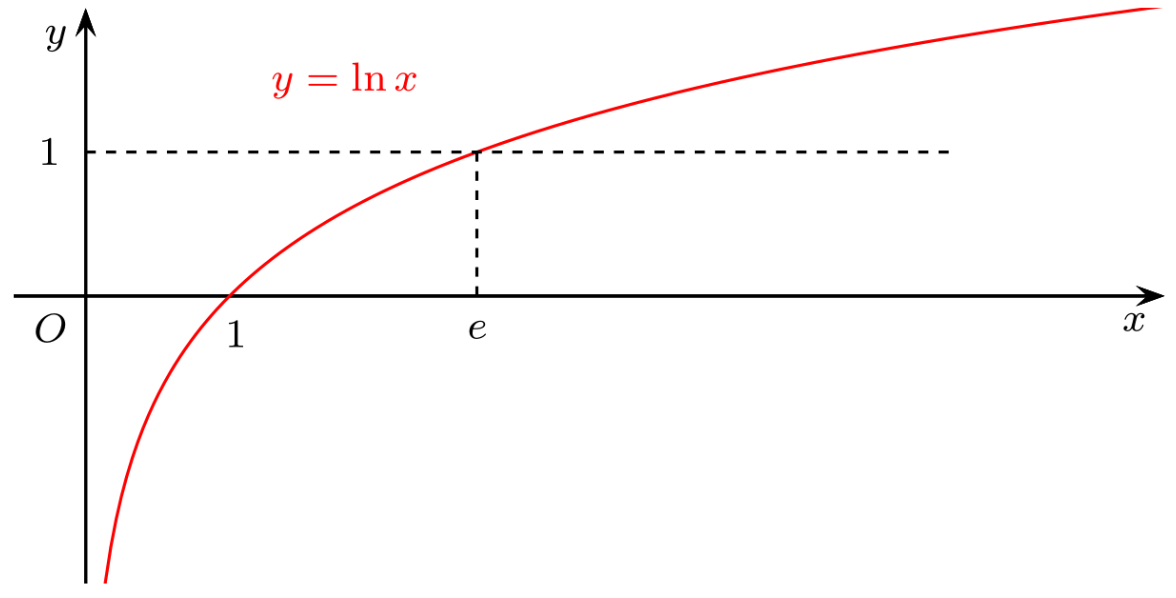
\includegraphics[width=0.4\linewidth]{ma1102r-natural-logarithm-1.png}
    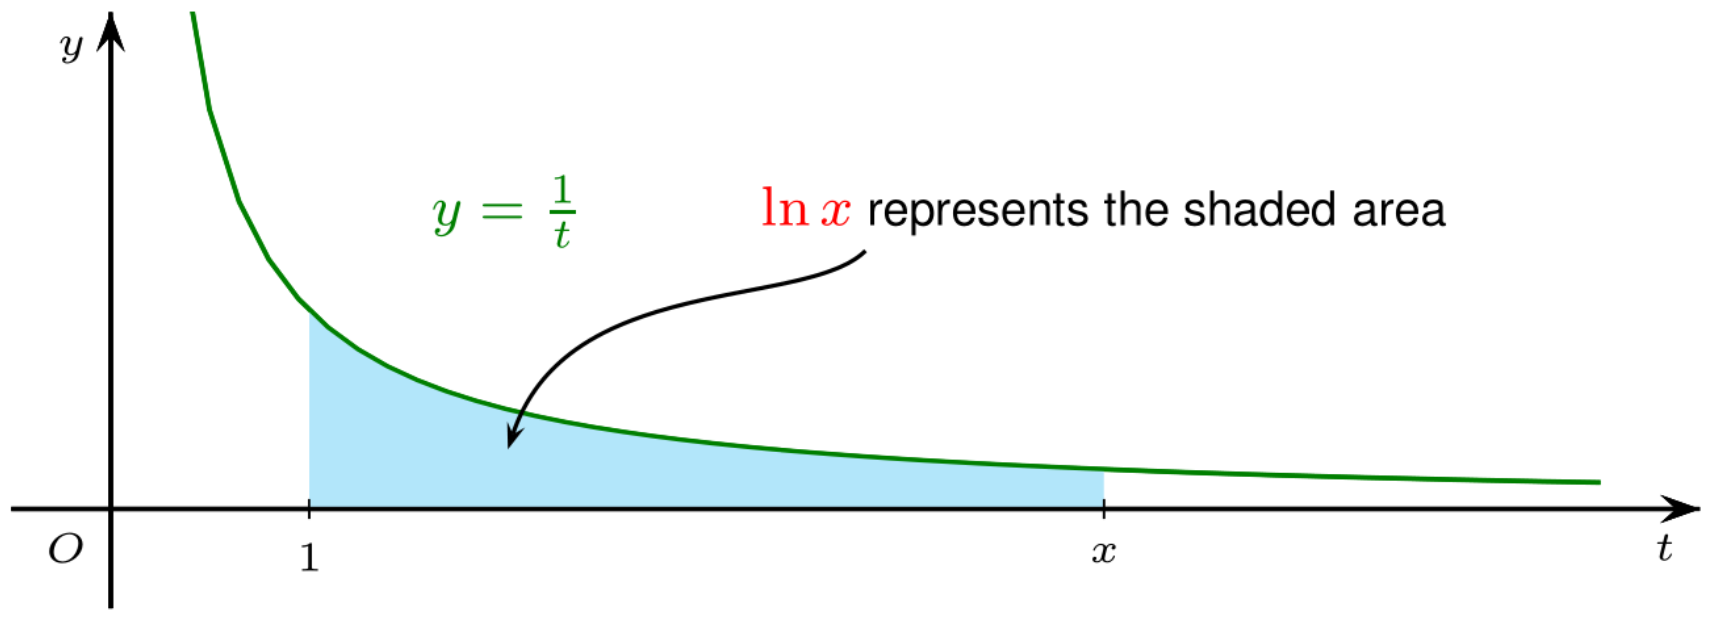
\includegraphics[width=0.55\linewidth]{ma1102r-natural-logarithm-2.png}
\end{center}
\begin{itemize}
    \item $\ln x < 0$ for $0 < x < 1$; $\quad \ln x > 0$ for $ > 1$; $\quad \ln 1 = 0$
    \item $\ln x$ is increasing on $\mathbb{R}^n$ ($\frac{d}{dx} \ln x > 0$)
\end{itemize}

\subsection{logarithmic differentiation I}
aka take $\ln$ on both sides and implicitly differentiate
\begin{center}
    for $y = f_1(x)f_2(x)\cdots f_n(x)$ (product of nonzero functions), 
    $\ln \abs{y} = \ln \abs{f_1(x)} + \ln \abs{f_2(x)} + \cdots + \ln \abs{f_n(x)}$
    \\* $\frac{dy}{dx} = \left[ \frac{f'_1(x)}{f_1(x)} + \frac{f'_2(x)}{f_2(x)} + \cdots + \frac{f'_n(x)}{f_n(x)} \right]y$
    \\* $= \left[ \frac{f'_1(x)}{f_1(x)} + \frac{f'_2(x)}{f_2(x)} + \cdots + \frac{f'_n(x)}{f_n(x)} \right]f_1(x)f_2(x)\cdots f_n(x)$
\end{center}

\subsection{logarithmic differentiation II}
\begin{center}
    for $y = f(x)^{g(x)} (f(x) > 0)$,
    \\* $\ln y = g(x) \ln f(x) \then \frac{dy}{dx} = y \frac{d}{dx}[g(x) \ln f(x)]$
    \begin{align*}
        \lim_{x \to a}(f(x)^{g(x)}) &= \lim_{x \to a} \exp \left( g(x) \ln f(x) \right) \\
        &= \exp\left( \lim_{x \to a} g(x) \ln f(x) \right)
    \end{align*}
\end{center}

\subsection{exponential function}
\begin{center}
    $y = e^x = \exp(x) \iff \ln y = x$
    \\* $\exp(x) = \ln ^{-1} (x)$ ($\exp(x)$ is the inverse of $\ln x$)
    \\* $a^x = \exp(x \ln a) = e^{x \ln a}$
    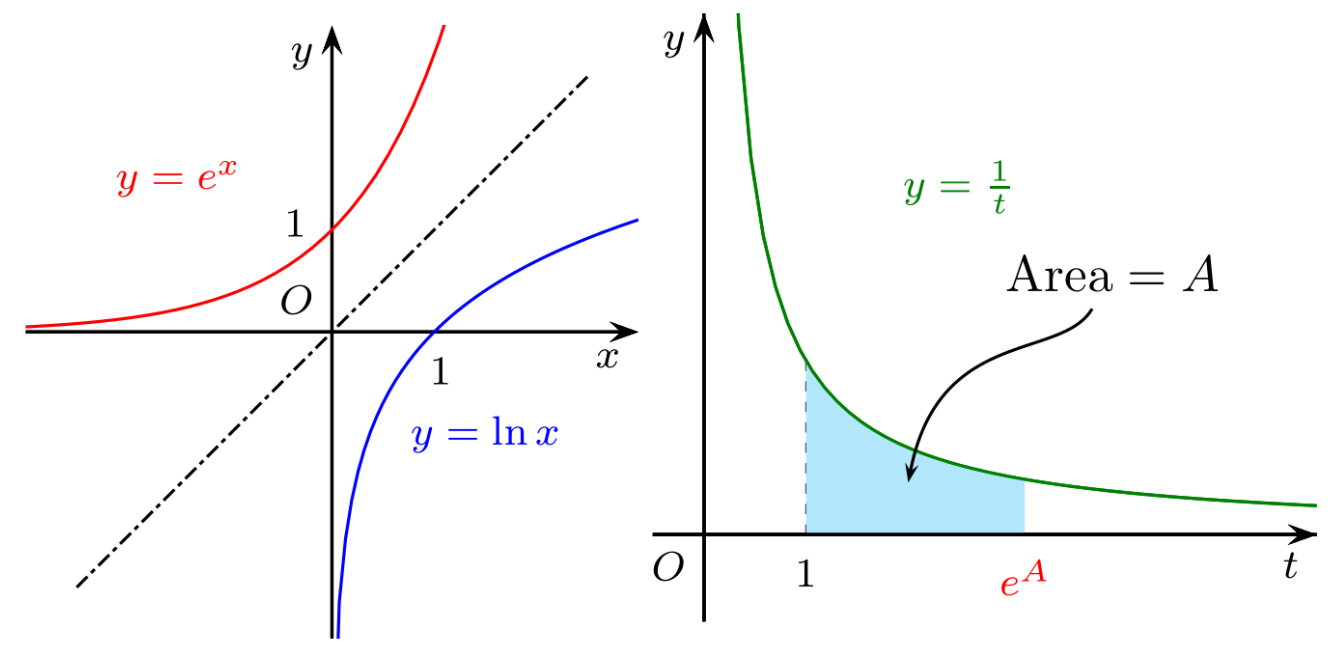
\includegraphics[width=0.8\linewidth]{ma1102r-exponential-function.png}
    \\* ${\displaystyle{e = \lim_{n \to \infty}(1 + \frac{1}{n})^n}}$
\end{center}
\begin{itemize}
    \item $\ln(e^x) = x$ for $x \in \mathbb{R}$ and $e^{\ln y} = y$ for $y \in \mathbb{R}^+$
    \item common equations
    \begin{itemize}
        \item ${\displaystyle{\lim_{x \to \infty} e^x =\infty}}$, ${\displaystyle{\lim_{x \to -\infty} e^x = 0}}$
        \item ${\displaystyle{\lim_{x \to \infty} \frac{e^x}{x^n} = \infty}}$ for $n \in \mathbb{Z}^+$
        \item ${\displaystyle{e^x = \sum^\infty_{n = 0} \frac{x^n}{n!} = 1 + x + \frac{x^2}{2!} + \frac{x^3}{3!} + \dots}}$
    \end{itemize}
\end{itemize}
\subsubsection{properties}
\begin{minipage}{0.32\linewidth}   
    \begin{itemize}
        \item $a^ua^v = a^{u+v}$
        \item $a^{-u} = \frac{1}{a^u}$
        \item $(a^u)^v = a^{uv}$
        \item $(a^x)' = a^x\ln a$
        \item $\frac{d}{dx} x^r = rx^{r-1}$
    \end{itemize}
\end{minipage}
\hfill\vline\hfill
\begin{minipage}{0.65\linewidth}
    \begin{itemize}
        \item ${\displaystyle{\lim_{x \to \infty} e^x =\infty}}$, ${\displaystyle{\lim_{x \to -\infty} e^x = 0}}$
        \item ${\displaystyle{\lim_{x \to \infty} \frac{e^x}{x^n} = \infty}}$ for $n \in \mathbb{Z}^+$
        \item ${\displaystyle{e^x = \sum^\infty_{n = 0} \frac{x^n}{n!} = 1 + x + \frac{x^2}{2!} + \dots}}$
    \end{itemize}
\end{minipage}
\begin{itemize}
    \item $\int x^r \dx = \begin{cases}
        \frac{x^{r+1}}{r+1} + C & \text{ if }r \neq -1, \\
        \ln x + C & \text{ if }r = -1,
        \end{cases}$
    \begin{itemize}
        \item if $r$ is irrational, then $x^r$ is only defined for $x \geq 0$.
    \end{itemize}
\end{itemize}

\subsection{hyperbolic trigonometric functions}
\begin{center}
    $\sinh x = \frac{e^x - e^{-x}}{2}, \quad (\sinh x)' = \cosh x$
    \\* $\cosh x = \frac{e^x + e^{-x}}{2}, \quad (\cosh x)' = \sinh x$
\end{center}
properties
\begin{itemize}
    \item $\cosh^2 x - \sinh^2 x = 1$
    \item parametrization represents a \textbf{hyperbola} - 
        \\* let $\begin{cases}
            x = \cosh t, \\ y = \sinh t.
        \end{cases}$ Then $x^2 - y^2 = 1$
\end{itemize}
\begin{minipage}{0.48\linewidth}   
    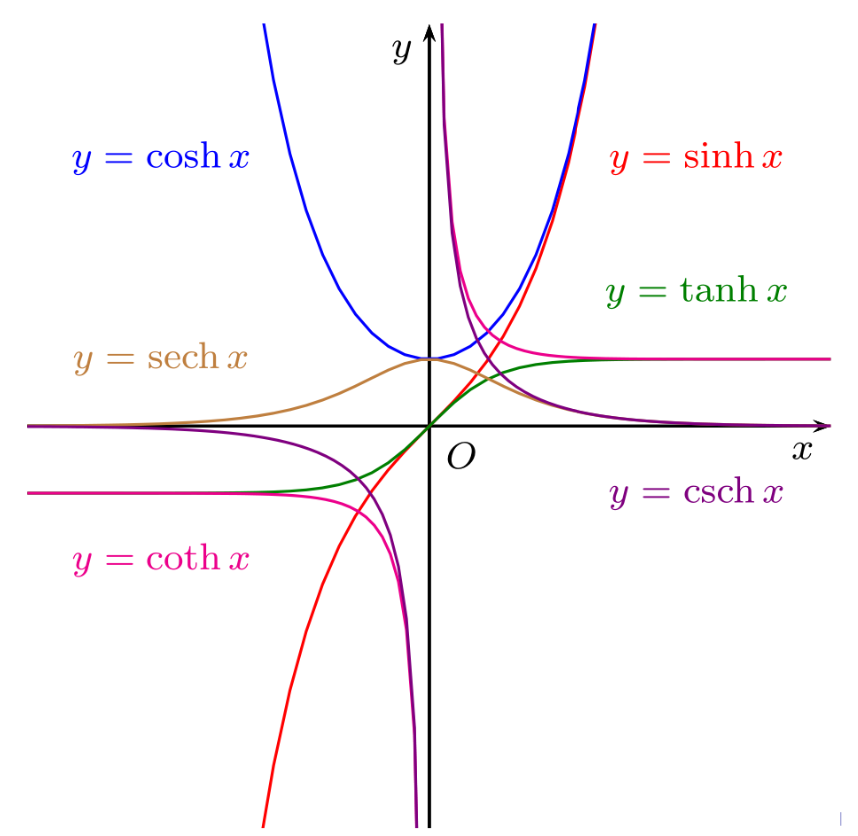
\includegraphics[width=0.98\linewidth]{ma1102r-hyperbolic-trigonometric-functions.png}
\end{minipage}
\begin{minipage}{0.5\linewidth}
    \begin{center}
        $\tanh x = \frac{\sinh x}{\cosh x}$
    \\* $\coth x = \frac{\cosh x}{\sinh x}$
    \\* $\mathop{sech} x = \frac{1}{\cosh x}$
    \\* $\mathop{csch} x = \frac{1}{\sinh x}$
    \\ \ 
    \\ inverse hyperbolic functions:
    \\* $\sinh^{-1}x = y \Leftrightarrow x = \sinh y$
    \\* $\cosh^{-1}x = y \Leftrightarrow x = \cosh y$
    \end{center}
\end{minipage}
\begin{itemize}
    \item properties
    \begin{itemize}
        \item $\frac{d}{dx} \sinh^{-1}x = \frac{1}{\sqrt{x^2 + 1}}$
        \item $\frac{d}{dx} \cosh^{-1}x = \frac{1}{\sqrt{x^2 - 1}}$
        \item $\sinh^{-1} x = \ln(x + \sqrt{x^2 + 1}), x \in \mathbb{R}$ 
        \item $\cosh^{-1} x = \ln(x + \sqrt{x^2 - 1}), x \geq 1$ 
        \item $\tanh^{-1} x = \frac{1}{2} \ln(\frac{1+x}{1-x}), \quad -1 < x < 1$
    \end{itemize}
\end{itemize}

\section{07. APPLICATIONS OF INTEGRALS}
\subsection{volume} 
\begin{center}
    \begin{multicols}{2}
        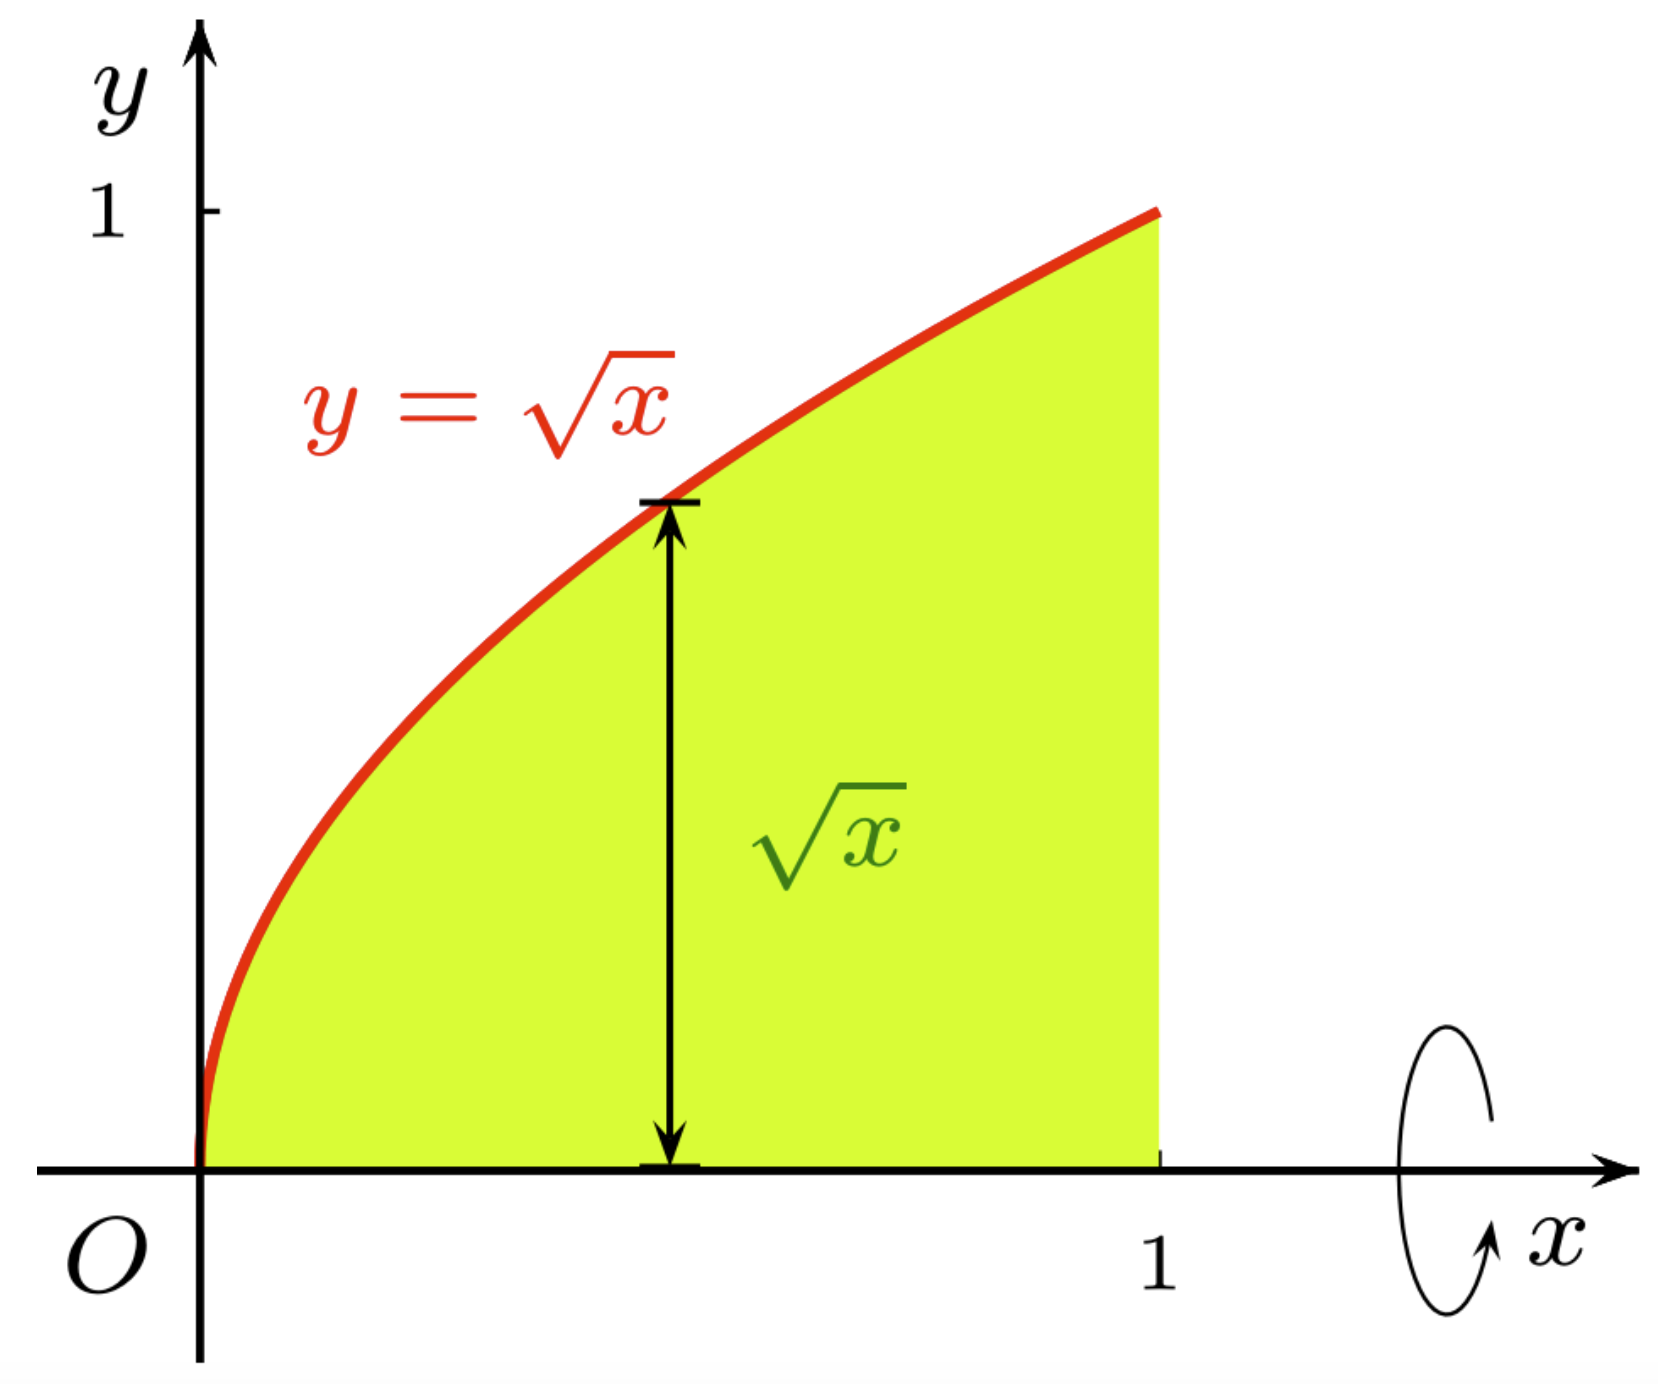
\includegraphics[width=0.95\linewidth]{ma1102r-volume-revolution-x.png}
        \\ rotate about the \textbf{x-axis}:
        \\* ${\displaystyle{V = \pi \int^b_a (f(x))^2 \dx}}$
        
        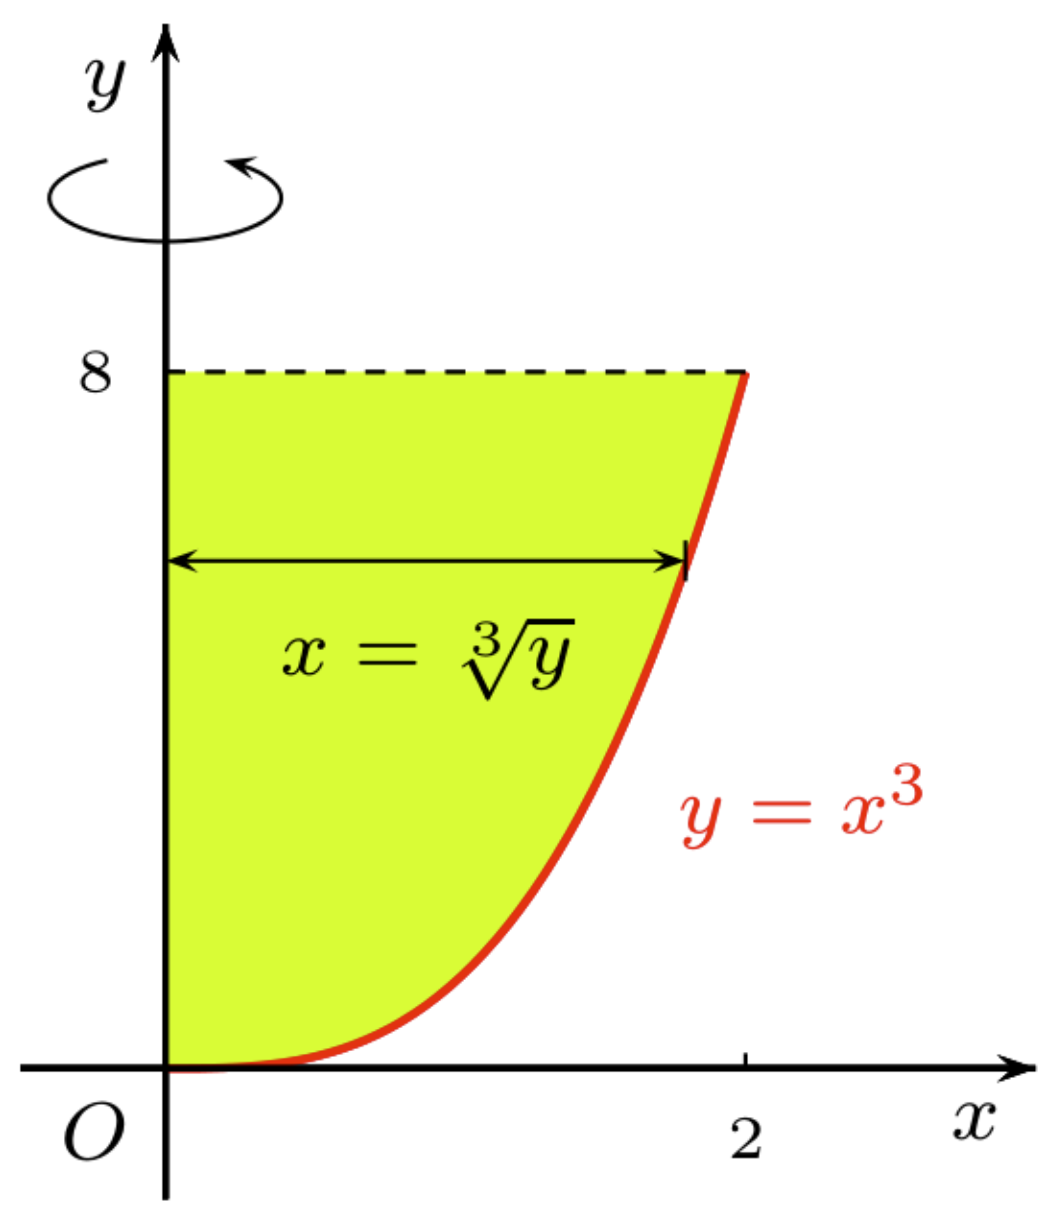
\includegraphics[width=0.7\linewidth]{ma1102r-volume-revolution-y.png}
        \\ rotate about the \textbf{y-axis}: 
        \\* ${\displaystyle{V = \pi \int^b_a (f(y))^2 \mathop{dy}}}$
    \end{multicols}
\end{center}

\subsubsection{method of cylindrical shells}
\begin{center}
    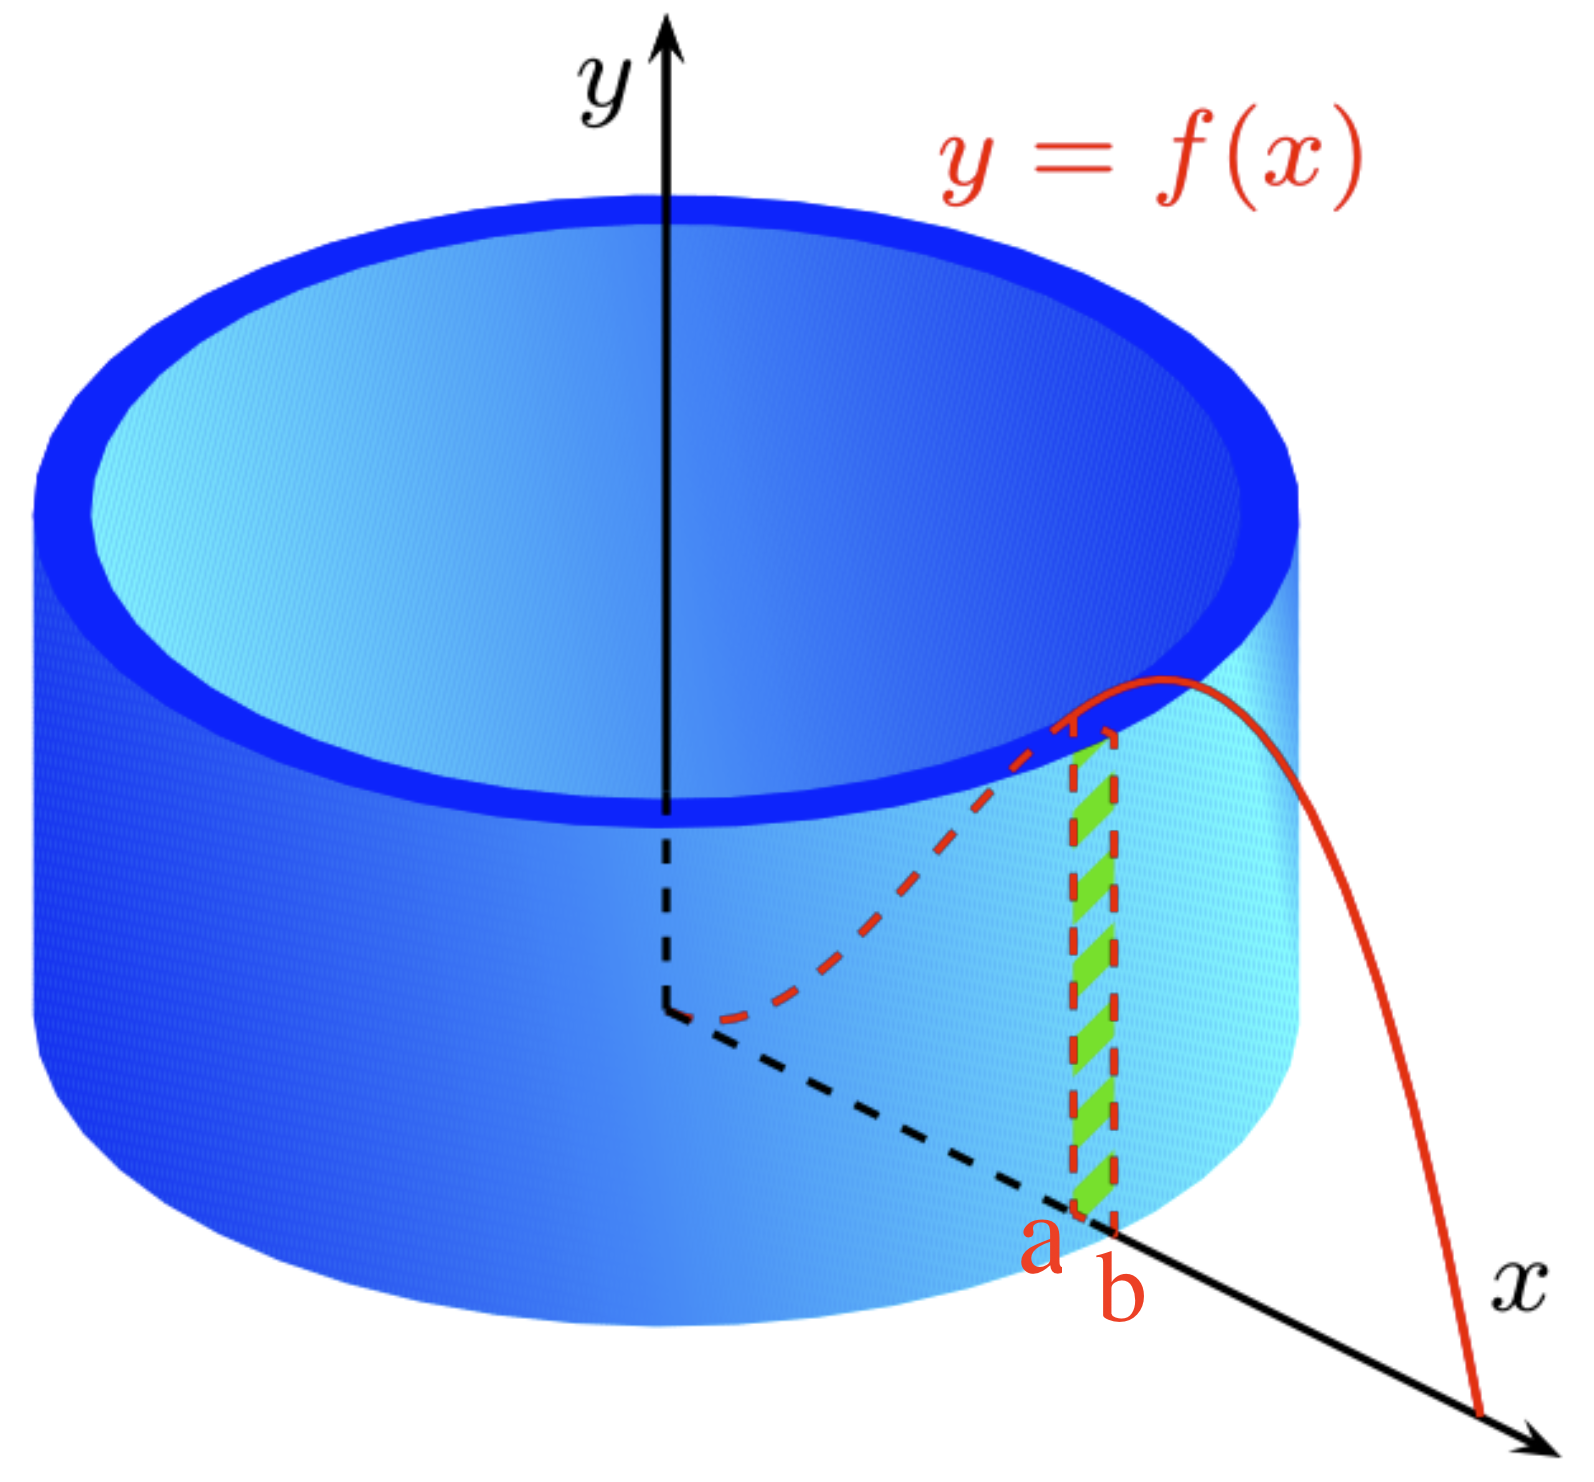
\includegraphics[width=0.4\linewidth]{ma1102r-volume-revolution-cylindrical.png}
    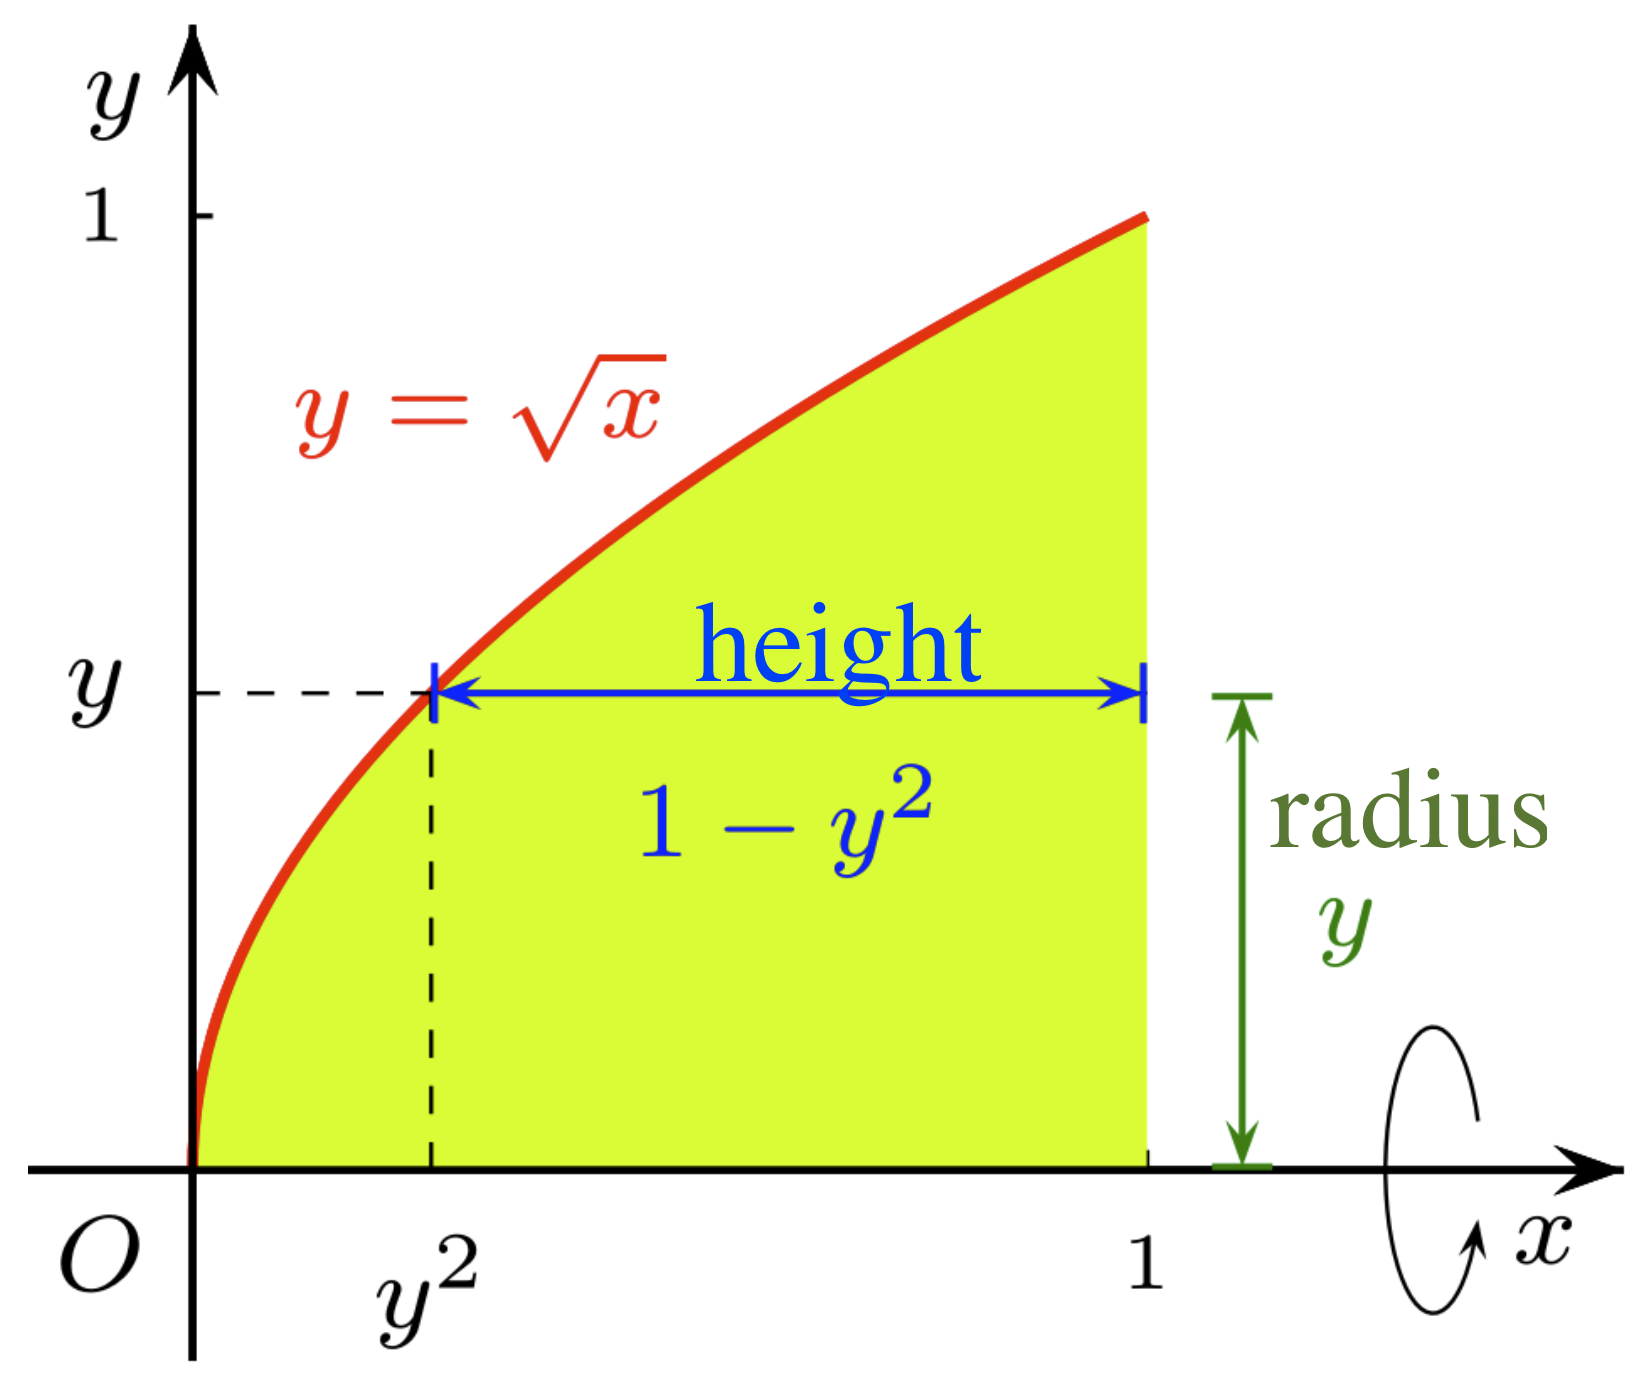
\includegraphics[width=0.4\linewidth]{ma1102r-volume-revolution-cylindrical-y.png}
    \\ rotation about \textbf{x-axis}:
        \\* $V = \int^b_a 2\pi x f(x) \dx = \int 2\pi (radius \cdot height) \dx$
    \\ rotation about \textbf{y-axis}:
        \\* $V = \int^b_a 2\pi y f(y) \mathop{dy} = \int 2\pi (radius \cdot height) \mathop{dy}$
\end{center}

\subsection{arc length}
\begin{minipage}{0.25\linewidth}
    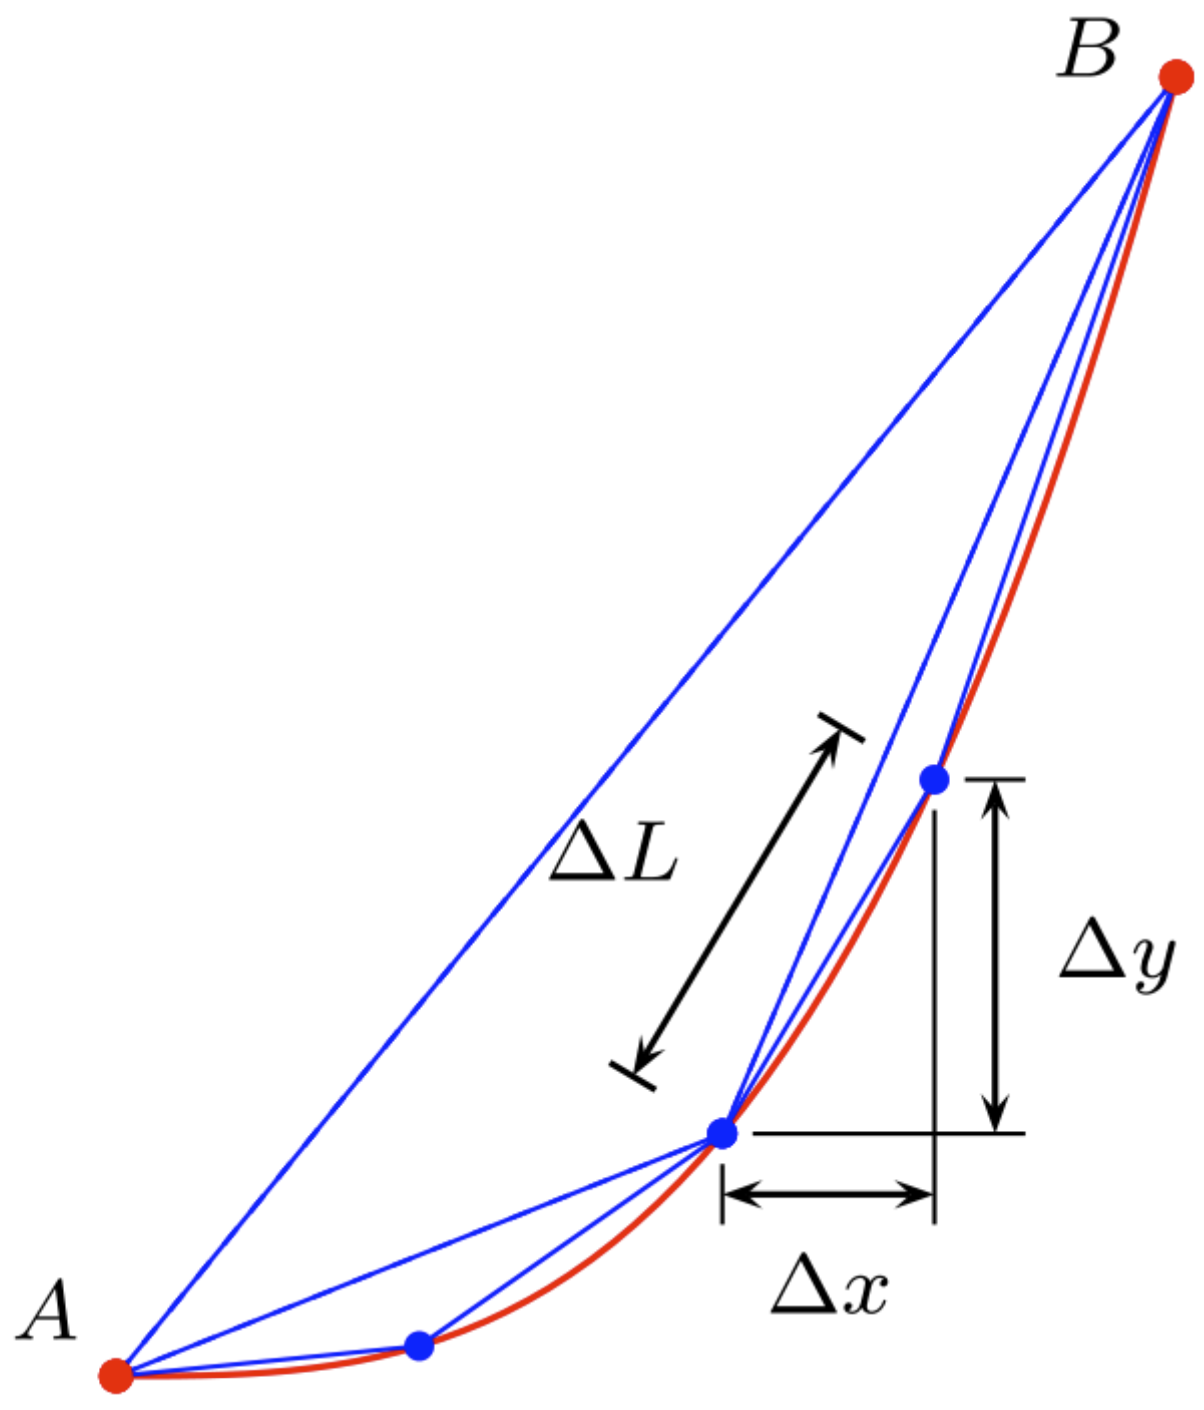
\includegraphics[width=0.95\linewidth]{ma1102r-arc-length.png}
\end{minipage}
\begin{minipage}{0.7\linewidth}
    \begin{itemize}
        \item a function $f$ is \textbf{smooth} if $f'$ is continuous.
        \item arc length, 
        \\ \noindent\fbox{%
        \parbox{0.9\linewidth}{%
        \begin{tightcenter}
            ${\displaystyle{L = \int^b_a \sqrt{1 + (f'(x))^2} \dx}}$
        \end{tightcenter}
        }
        }%
    \end{itemize}
\end{minipage}

\subsection{surface area of revolution}
\begin{center}
    Let $f$ be a smooth function such that $f(x) \geq 0$ on $[a, b]$. 
    \\ Then the area of the surface obtained by rotating the curve $y = f(x),  a \leq x \leq b$ about the $x$-axis is
    \noindent\fbox{%
    \parbox{0.9\linewidth}{%
    \begin{tightcenter}
        ${\displaystyle{A = \int^b_a 2\pi f(x) \sqrt{1 + (f'(x))^2} \dx}}$
    \end{tightcenter}
    }
    }%
\end{center}

\subsection{misc}
\subsubsection{triangle inequality}
\begin{center}
    $\abs{a + b} \leq \abs{a} + \abs{b}$ for all $a, b \in \mathbb{R}$
\end{center}

\subsubsection{binomial theorem}
\begin{center}
    $\displaystyle{(a+b)^n = \sum^n_{k=0}\binom{n}{k}a^{n-k}b^k}$
    \\* $= a^n + \binom{n}{1}a^{n-1}{b} + \dots + \binom{n}{n-1} ab^{n-1} + b^n$
\end{center}
\begin{center}
    where the binomial coefficient is given by 
    \\* $\binom{n}{k} = \frac{n!}{k!(n-k)!}$
\end{center}

\subsubsection{factorisation}
\begin{center}
    $a^n-b^n = (a-b)(a^{n-1} + a^{n-2}b + \cdots + ab^{n-2} + b^{n-1})$
    $a^3-b^3 = (a-b)(a^2+ab+b^2)$
    $a^3+b^3 = (a+b)(a^2-ab+b^2)$
\end{center}

\subsubsection{misc}
\begin{itemize}
    \item $\forall x \in (0, \frac{\pi}{2}), \sin x < x < \tan x$
\end{itemize}

\end{multicols}

\end{document}